\documentclass[a4paper,12pt]{report}

\usepackage[utf8]{inputenc}
\usepackage[a4paper,margin=24mm]{geometry}
\usepackage[skip=10pt plus1pt, indent=20pt]{parskip}
\usepackage[colorlinks=true,allcolors=blue,urlcolor=magenta]{hyperref}

\usepackage{caption}
\usepackage{indentfirst,setspace,subcaption}
\usepackage{amsmath,amssymb,graphicx,xcolor,url}
\usepackage{fancyhdr,tocbasic,titlesec,minted,listings}
\usepackage{algorithm}
\usepackage{algpseudocode}
\usepackage{float}


\renewcommand{\thesection}{\arabic{section}}

\renewcommand{\thesection}{\arabic{section}}
\renewcommand{\listoflistingscaption}{Source code}

\newcommand{\codeimport}{\inputminted[breakanywhere=true,breaklines=true]}


% Code highlighting
\usemintedstyle{one-dark}
\setminted{frame=lines,
  framesep=2mm,
  baselinestretch=1.2,
  fontsize=\footnotesize,
  linenos,
  breakanywhere,
  breaklines,
  mathescape
}

% Header and footer styling
\pagestyle{fancy}
\setlength{\headheight}{18pt}
\fancyhf{}
\fancyhead[R]{\nouppercase\rightmark\hfill~Project 03: Decision Tree}
\fancyfoot[C]{\hfill\thepage\hfill}

% TOC styling
\DeclareTOCStyleEntry[
  indent=12pt,
  level=1
]{largetocline}{section}

% Title page data
\title{Project 03: Decision Tree}
\author{\begin{tabular}{r c}
  Ngo Nguyen The Khoa & 23127065\\
  Bui Minh Duy       & 23127040\\
  Nguyen Le Ho Anh Khoa      & 23127211\\
\end{tabular}}
\date{April 5, 2025}

\begin{document}
\newenvironment{codewithlisting}[2]{
	\begin{listing}[!ht]
		\caption[#1]{#1}
		\label{listing:#2}}{\end{listing}
}


% Title page and TOC
\thispagestyle{empty}
\begin{titlepage}
	\begin{center}
		\makeatletter
		\newcommand{\HRule}{\rule{\linewidth}{0.4mm}}

		\textsc{\LARGE Vietnam National University,\\Ho Chi Minh City}\\[1.5cm]
		\textsc{\Large University of Science}\\[0.5cm]
		\textsc{\Large Faculty of Information Technology}\\[1.5cm]

		{\HRule}\\[1cm]
		{\huge \bfseries \@title}\\[0.5cm]
		{\HRule}\\[2cm]

		\textsc{\large CS14003 --  Introduction to Artificial Intelligence}\\[0.5cm]

		\vfill\vfill\vfill

		{\large \@author}\\[1.5cm]
		{\large \@date}
		\makeatother
	\end{center}
\end{titlepage}

\tableofcontents\thispagestyle{empty}

% Report contents
\pagebreak
\section{Group Information}
\begin{itemize}
  \item \textbf{Subject:} Introduction to Artificial Intelligence.
  \item \textbf{Class:} 23CLC09.
  \item \textbf{Lecturer:} Bui Duy Dang, Le Nhut Nam.
  \item \textbf{Team members:}
        \begin{center}
          \renewcommand{\arraystretch}{1.5}
          \begin{tabular}{|c|l|c|l|}
            \hline
            \textbf{No.} & \textbf{Fullname}     & \textbf{Student ID} & \textbf{Email}                                                         \\\hline
            1            & Ngo Nguyen The Khoa   & 23127065            & \href{mailto:nntkhoa23@clc.fitus.edu.vn}{nntkhoa23@clc.fitus.edu.vn}   \\\hline
            2            & Bui Minh Duy          & 23127040            & \href{mailto:bmduy23@clc.fitus.edu.vn}{bmduy23@clc.fitus.edu.vn}       \\\hline
            3            & Nguyen Le Ho Anh Khoa & 23127211            & \href{mailto:nlhakhoa23@clc.fitus.edu.vn}{nlhakhoa23@clc.fitus.edu.vn} \\\hline
          \end{tabular}
        \end{center}
\end{itemize}

\section{Project Information}
\begin{itemize}
  \item \textbf{Name:} Decision Tree Classifier using Scikit-learn.
  \item \textbf{Developing Environment:} Visual Studio Code (Windows, WSL).
  \item \textbf{Programming Language:} Python.
  \item \textbf{Libraries and Tools:}
        \begin{itemize}
          \item \textbf{Libraries:}
                \begin{itemize}
                  \item \href{https://scikit-learn.org/stable/}{\textbf{scikit-learn:}} Machine learning library for training and evaluating decision tree models.
                  \item \href{https://pandas.pydata.org/}{\textbf{pandas:}} Data manipulation and analysis.
                  \item \href{https://numpy.org/}{\textbf{numpy:}} Numerical operations.
                  \item \href{https://matplotlib.org/}{\textbf{matplotlib}}, \href{https://seaborn.pydata.org/}{\textbf{seaborn:}} Data visualization libraries.
                  \item \href{https://graphviz.org/}{\textbf{graphviz:}} Visualization of decision trees.
                \end{itemize}
          \item \textbf{Tools:}
                \begin{itemize}
                  \item \href{https://git-scm.com/}{\textbf{Git}}, \href{https://github.com/}{\textbf{GitHub}}: Source code version control.
                  \item \href{https://code.visualstudio.com/}{\textbf{Visual Studio Code}}: Code editor for Python, LaTeX.
                \end{itemize}
        \end{itemize}
  \item \textbf{Datasets:}
        \begin{itemize}
          \item \href{https://archive.ics.uci.edu/dataset/17/breast+cancer+wisconsin+diagnostic}{\textbf{Breast Cancer Wisconsin (Diagnostic)}}
          \item \href{https://archive.ics.uci.edu/dataset/186/wine+quality}{\textbf{Wine Quality}}
          \item \href{https://archive.ics.uci.edu/dataset/19/car+evaluation}{\textbf{Car Evaluation}}
        \end{itemize}
\end{itemize}


\pagebreak
\section{Work Assignment Table}
\begin{center}
  \renewcommand{\arraystretch}{1.5}
  \begin{tabular}{|c|p{\dimexpr0.55\linewidth-2\tabcolsep}|r|c|}
    \hline
    \textbf{No.} & \textbf{Task Description}                                                                                                 & \textbf{Assigned to} & \textbf{Rate} \\\hline
    1            & Prepare all three datasets (Breast Cancer, Wine Quality, and Additional) with proper preprocessing and stratified splits. & The Khoa             & 100\%         \\\hline
    2            & Implement and train decision tree models for each dataset with different train/test splits.                               & Minh Duy             & 100\%         \\\hline
    3            & Visualize decision trees using Graphviz.                                                                                  & Anh Khoa             & 100\%         \\\hline
    4            & Evaluate classifiers with classification reports and confusion matrices.                                                  & Anh Khoa             & 100\%         \\\hline
    5            & Analyze impact of tree depth on accuracy (80/20 split, varying max\_depth values).                                        & The Khoa             & 100\%         \\\hline
    6            & Research and integrate additional dataset.                                                                                & Minh Duy             & 100\%         \\\hline
    7            & Conduct comparative analysis across the three datasets.                                                                   & The Khoa             & 100\%         \\\hline
    8            & Visualize and format results (accuracy tables, charts, dataset distributions, etc.).                                      & Anh Khoa             & 100\%         \\\hline
    9            & Write and format final report with all results, insights, and figures.                                                    & Minh Duy             & 100\%         \\\hline
    10           & Ensure overall cohesion, proofreading, and prepare final PDF submission.                                                  & All                  & 100\%         \\\hline
  \end{tabular}
\end{center}

\section{Self-evaluation}
\begin{center}
  \renewcommand{\arraystretch}{1.5}
  \begin{tabular}{|c|p{\dimexpr0.82\linewidth-2\tabcolsep}|c|}
    \hline
    \textbf{No.} & \textbf{Task Description}                                                                  & \textbf{Rate} \\\hline
    1            & Prepare datasets with stratified splits and visualize class distributions.                 & 100\%         \\\hline
    2            & Train and visualize decision tree models on all datasets using multiple train/test splits. & 100\%         \\\hline
    3            & Evaluate decision trees using classification reports and confusion matrices.               & 100\%         \\\hline
    4            & Analyze the impact of decision tree depth on model accuracy.                               & 100\%         \\\hline
    5            & Research and integrate an additional dataset for training and evaluation.                  & 100\%         \\\hline
    6            & Conduct comparative analysis across all datasets.                                          & 100\%         \\\hline
    7            & Create charts, tables, and visualizations to support findings.                             & 100\%         \\\hline
    8            & Write and format the final report with insights and well-organized results.                & 100\%         \\\hline
    9            & Team collaboration and adherence to project schedule.                                      & 100\%         \\\hline
  \end{tabular}
\end{center}


\pagebreak
\section{Dataset Analysis and Experiments}
\subsection{Dataset Preparation and Preprocessing}
\begin{minted}{py}
def split_and_visualize(X, y, dataset_name: str):
    splits = {}

    for ratio in [0.4, 0.6, 0.8, 0.9]:
        X_train, X_test, y_train, y_test = train_test_split(
            X, y, train_size=ratio, stratify=y, shuffle=True, random_state=42
        )

        splits[ratio] = (X_train, X_test, y_train, y_test)

    return splits
\end{minted}
\begin{flushleft}
	To shuffle the dataset and ensure it is split in a stratified fashion, we use the \texttt{train\_test\_split} function from \texttt{sklearn.model\_selection}. The function takes the dataset and the target variable as inputs, along with the desired train-test split ratio.
	\begin{itemize}
		\item The \texttt{shuffle} parameter randomizes the order of the samples before splitting.
		\item The \texttt{stratify} parameter ensures the dataset is split in a stratified fashion.
	\end{itemize}
\end{flushleft}

\subsection{Interpreting Classification Report and Confusion Matrix}
\begin{minted}{py}
def train_evaluate_decision_tree(
    X_train,
    y_train,
    X_test,
    y_test,
    dataset_name: str,
    split_ratio,
):
    # Dynamically set feature and class names
    feature_names = X_train.columns.tolist()
    class_names = [str(cls) for cls in np.unique(y_train)]

    # Train model
    clf = DecisionTreeClassifier(criterion="entropy", random_state=42)
    clf.fit(X_train, y_train)

    # Predictions
    y_pred = clf.predict(X_test)

    # Classification Report (with validation)
    print(f"\nClassification Report ({dataset_name}, {display_ratio(split_ratio)}):")
    print(
        classification_report(
            y_test,
            y_pred,
            target_names=class_names,
            labels=np.unique(y_test),  # Ensure alignment with actual classes
        )
    )

    # Confusion Matrix
    sns.heatmap(
        confusion_matrix(y_test, y_pred),
        annot=True,
        fmt="d",
        xticklabels=class_names,
        yticklabels=class_names,
    )
\end{minted}
\begin{flushleft}
	To generate the classification report and confusion matrix:
	\begin{itemize}
		\item The \texttt{classification\_report} function provides a detailed report of the model's performance, including precision, recall, and F1-score for each class.
		\item The \texttt{confusion\_matrix} function generates a matrix that shows the number of correct and incorrect predictions for each class.
	\end{itemize}
\end{flushleft}

%================ Breast Cancer =================%
\clearpage
\subsection{Breast Cancer Wisconsin Dataset}
\subsubsection*{Dataset Description}
\begin{itemize}
	\item \textbf{Description:} The UCI Breast Cancer Wisconsin (Diagnostic) dataset is used for classifying tumors as malignant or benign based on features derived from its imaging data.
	\item \textbf{Dataset Info:} 569 samples, binary labels (malignant vs.\ benign), 30 numeric features.
	\item \textbf{Preprocessing:} shuffle \& stratified split at 40/60, 60/40, 80/20, 90/10.
\end{itemize}

\begin{figure}[H]
	\centering
	\begin{subfigure}{0.45\textwidth}
		\centering
		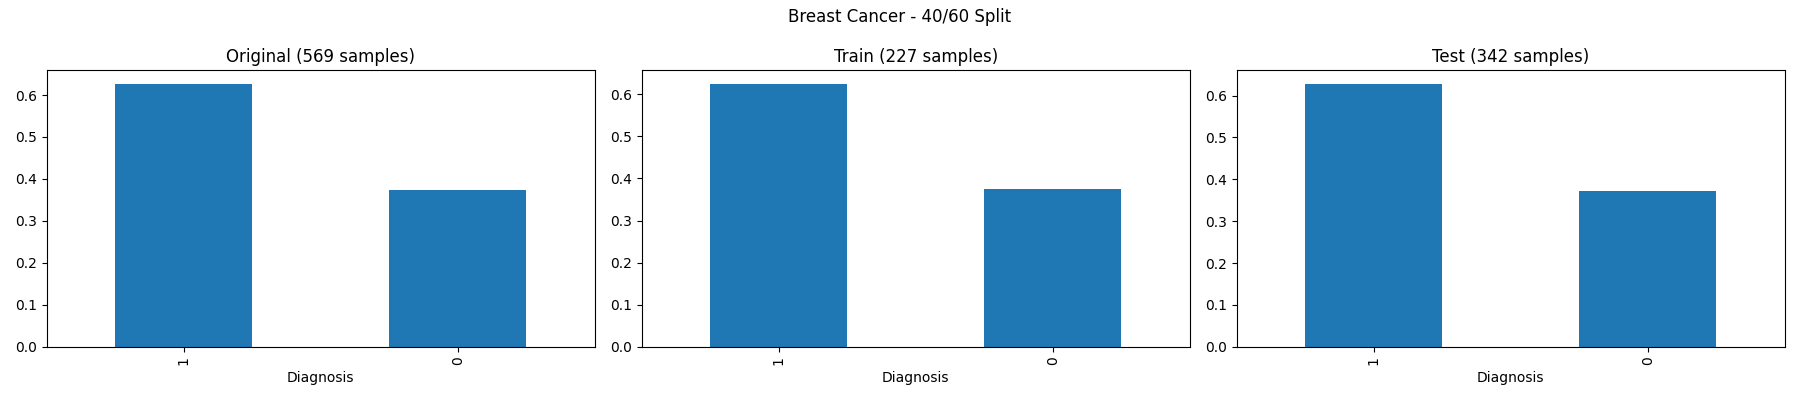
\includegraphics[width=\textwidth]{imgs/class_dist/class_dist__breast_cancer__40_vs_60.png}
		\caption{Breast Cancer: class distribution (40/60 split).}\label{fig:bc-cd-40-60}
	\end{subfigure}
	\hfill
	\begin{subfigure}{0.45\textwidth}
		\centering
		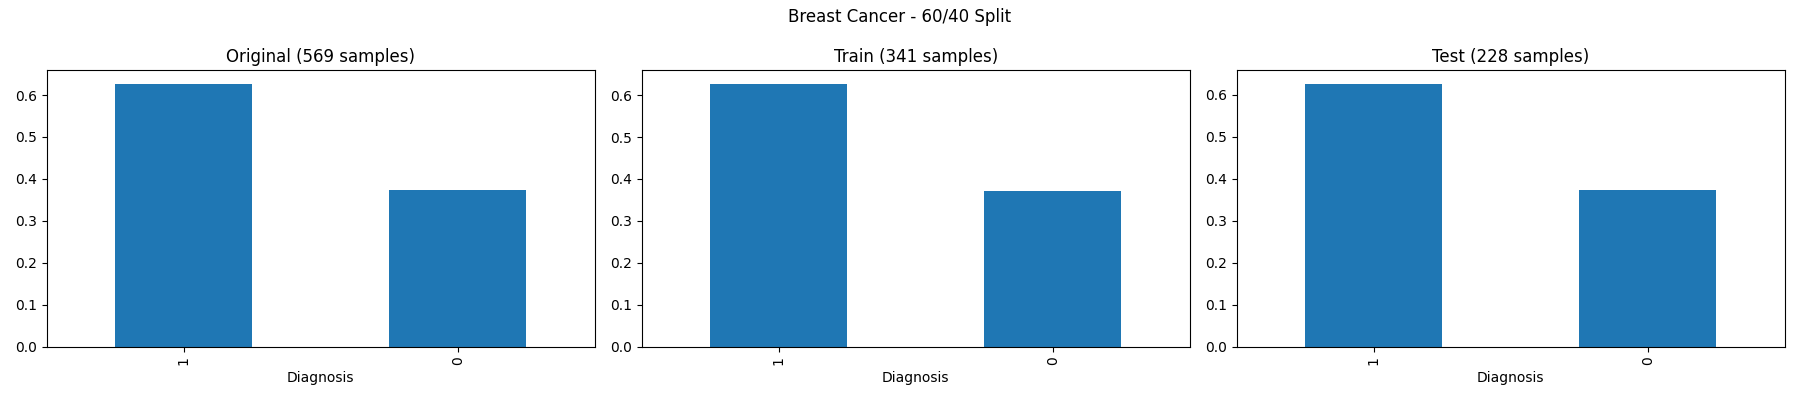
\includegraphics[width=\textwidth]{imgs/class_dist/class_dist__breast_cancer__60_vs_40.png}
		\caption{Breast Cancer: class distribution (60/40 split).}\label{fig:bc-cd-60-40}
	\end{subfigure}
	\hfill
	\begin{subfigure}{0.45\textwidth}
		\centering
		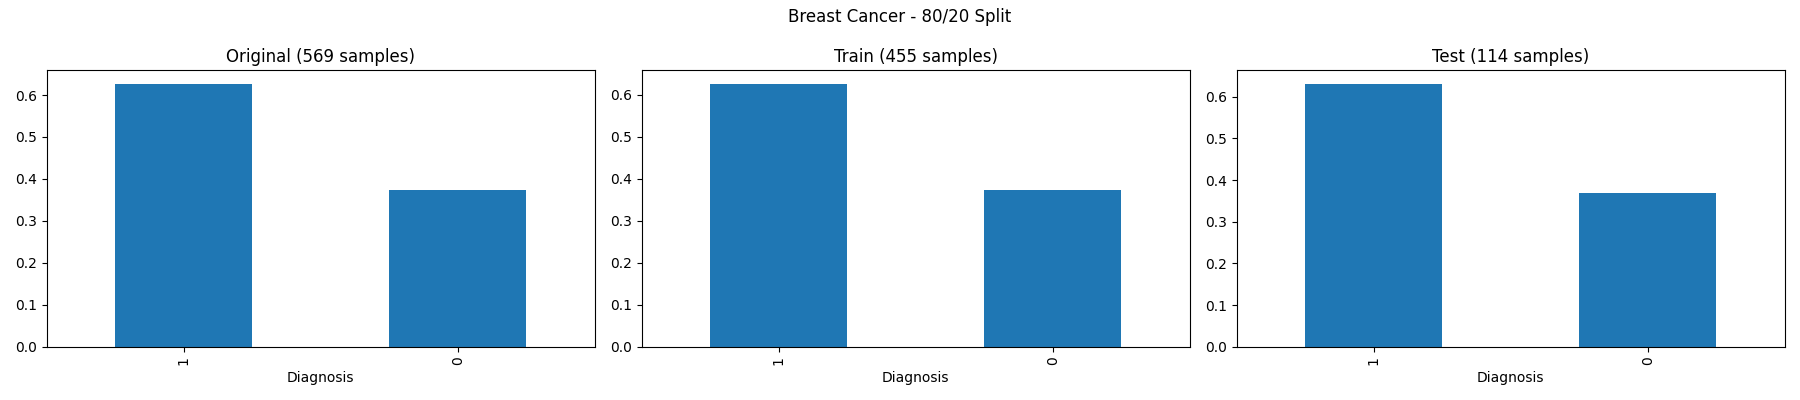
\includegraphics[width=\textwidth]{imgs/class_dist/class_dist__breast_cancer__80_vs_20.png}
		\caption{Breast Cancer: class distribution (80/20 split).}\label{fig:bc-cd-80-20}
	\end{subfigure}
	\hfill
	\begin{subfigure}{0.45\textwidth}
		\centering
		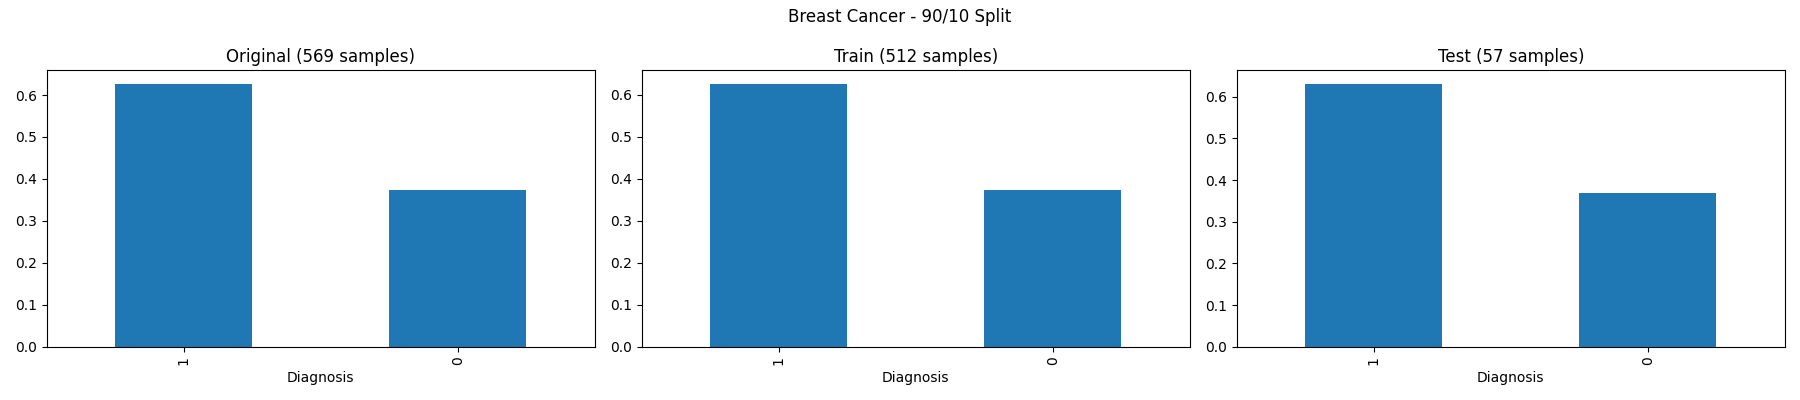
\includegraphics[width=\textwidth]{imgs/class_dist/class_dist__breast_cancer__90_vs_10.png}
		\caption{Breast Cancer: class distribution (90/10 split).}\label{fig:bc-cd-90-10}
	\end{subfigure}

	\caption{Class distributions}\label{fig:bc-cd-all}
\end{figure}

\clearpage
\subsubsection*{Building Decision Tree Classifiers for each train/test proportions}
\begin{figure}[H]
	\centering
	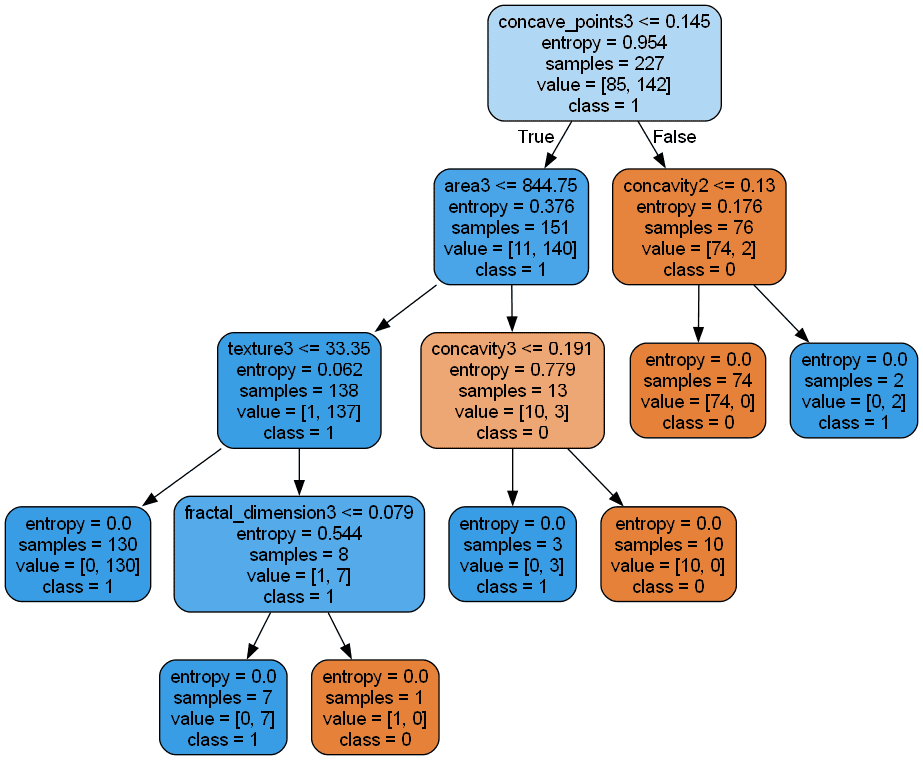
\includegraphics[width=0.65\textwidth]{imgs/dt-mini/dt__breast_cancer__40_vs_60.png}
	\caption{Breast Cancer: decision tree for 40/60 split.}\label{fig:bc-dt-40-60}
\end{figure}
\begin{figure}[H]
	\centering
	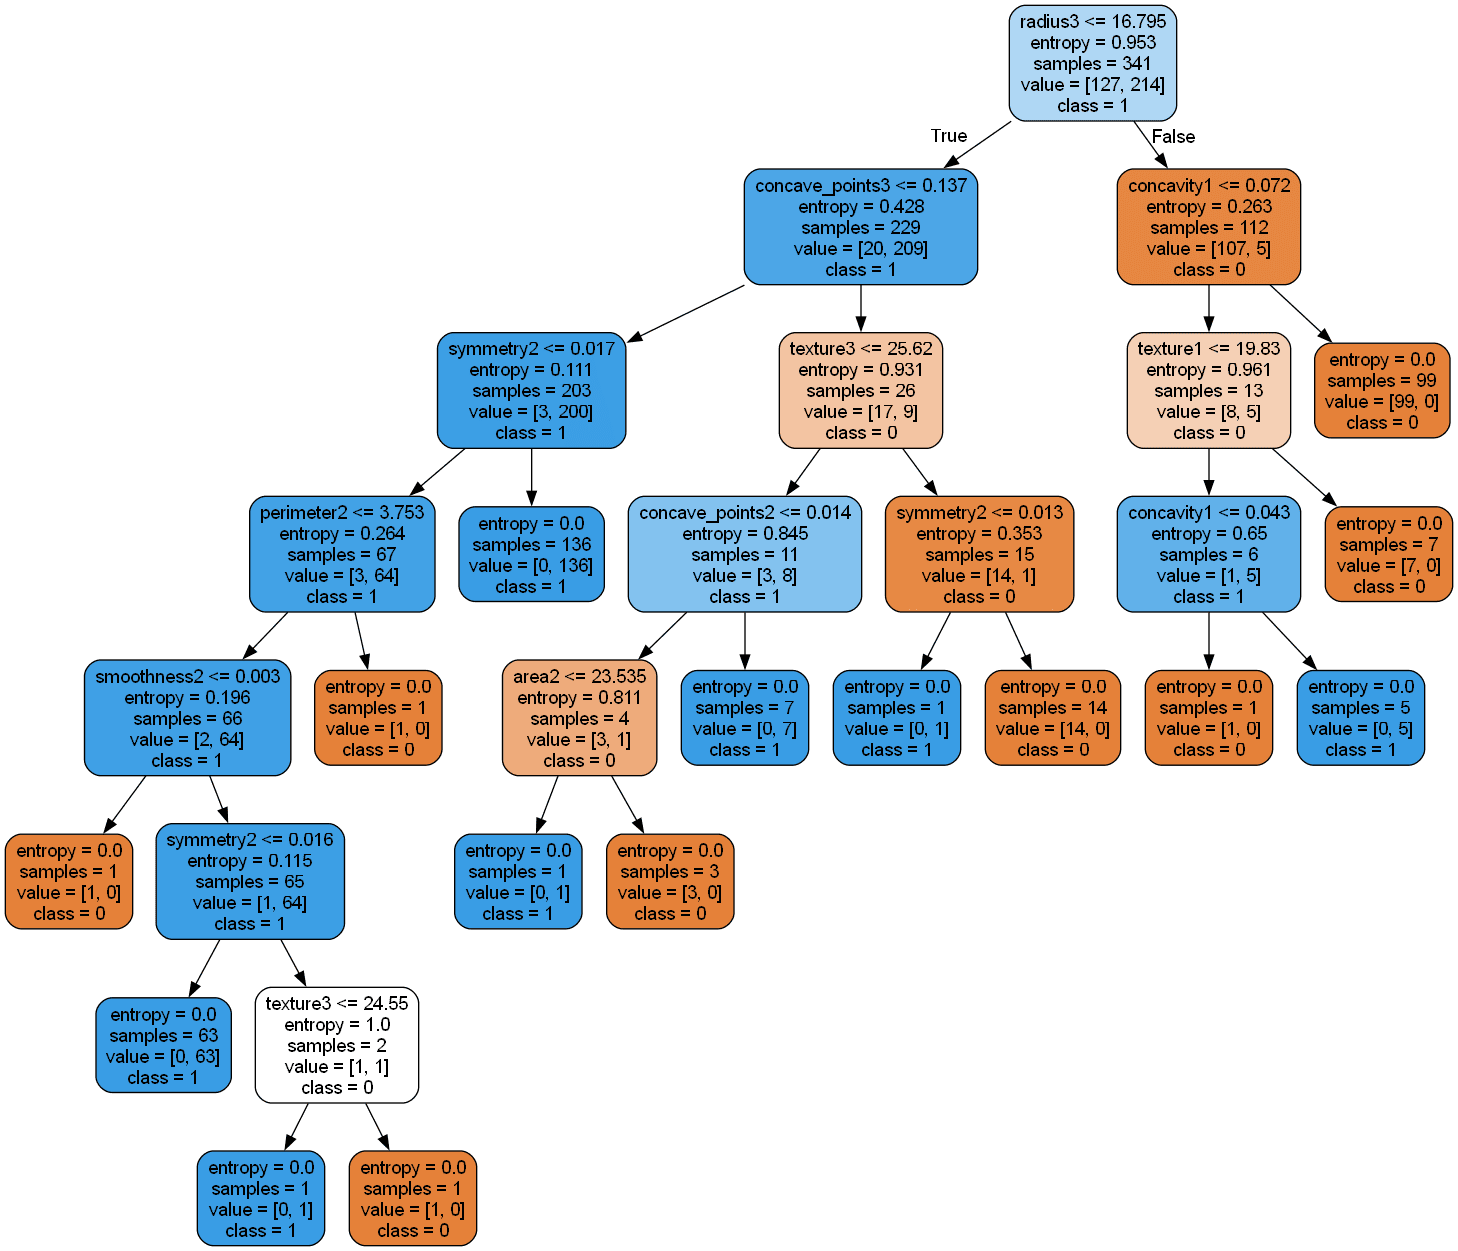
\includegraphics[width=0.65\textwidth]{imgs/dt-mini/dt__breast_cancer__60_vs_40.png}
	\caption{Breast Cancer: decision tree for 60/40 split.}\label{fig:bc-dt-60-40}
\end{figure}
\begin{figure}[H]
	\centering
	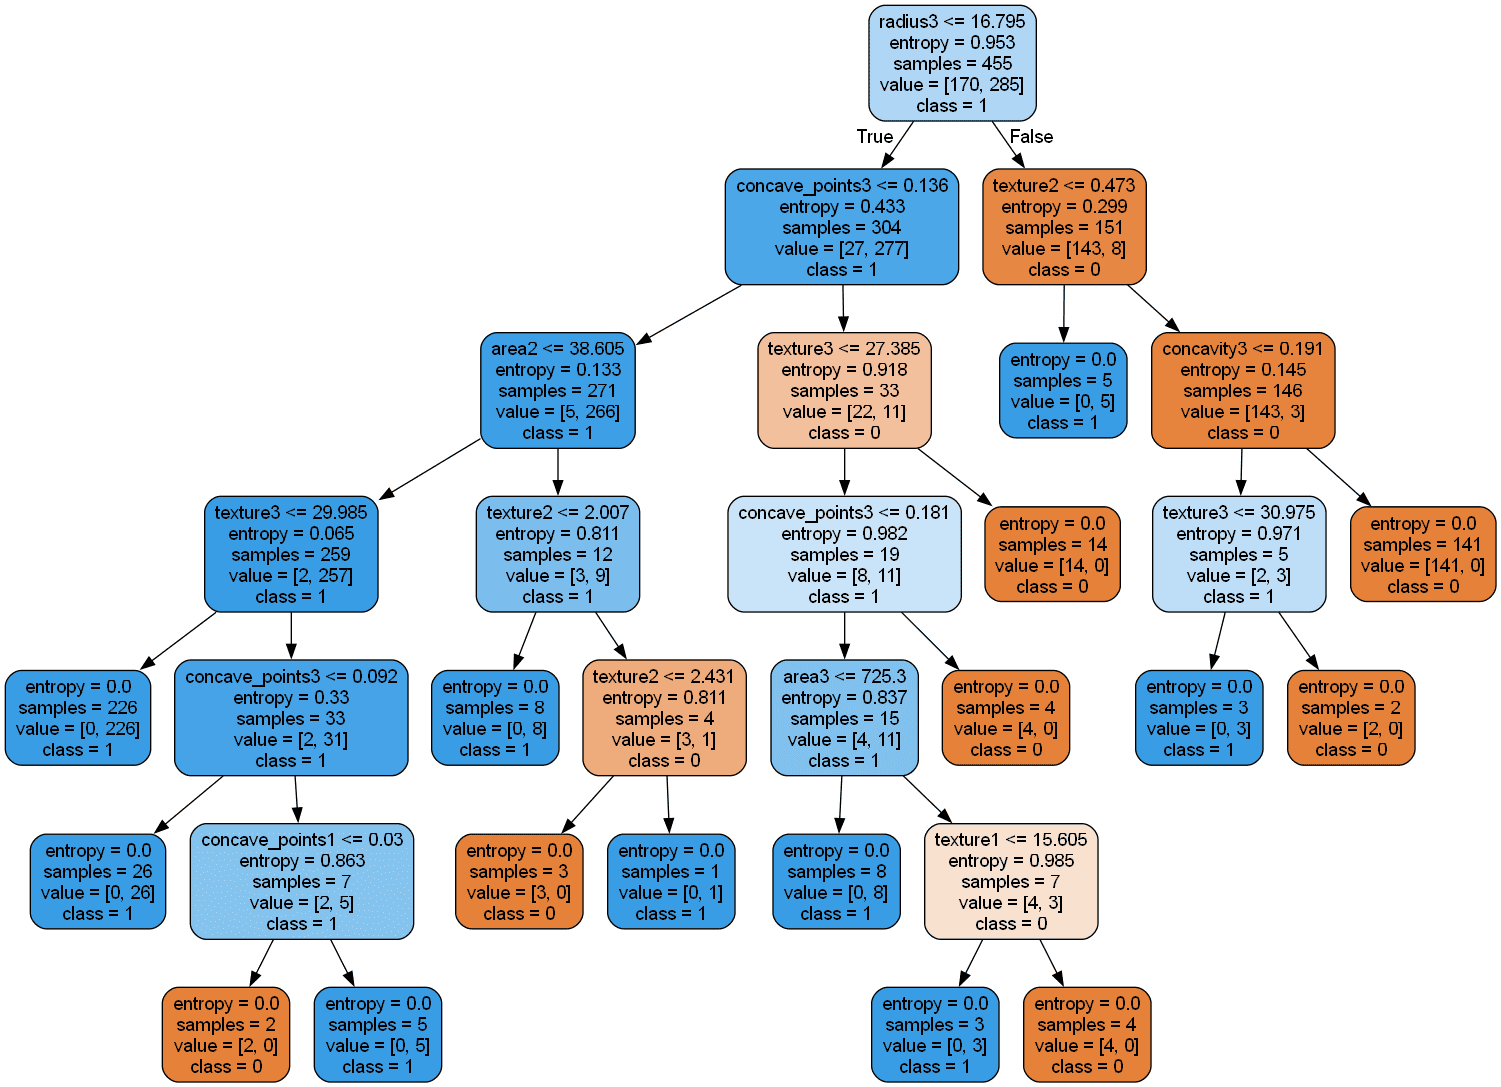
\includegraphics[width=0.65\textwidth]{imgs/dt-mini/dt__breast_cancer__80_vs_20.png}
	\caption{Breast Cancer: decision tree for 80/20 split.}\label{fig:bc-dt-80-20}
\end{figure}
\begin{figure}[H]
	\centering
	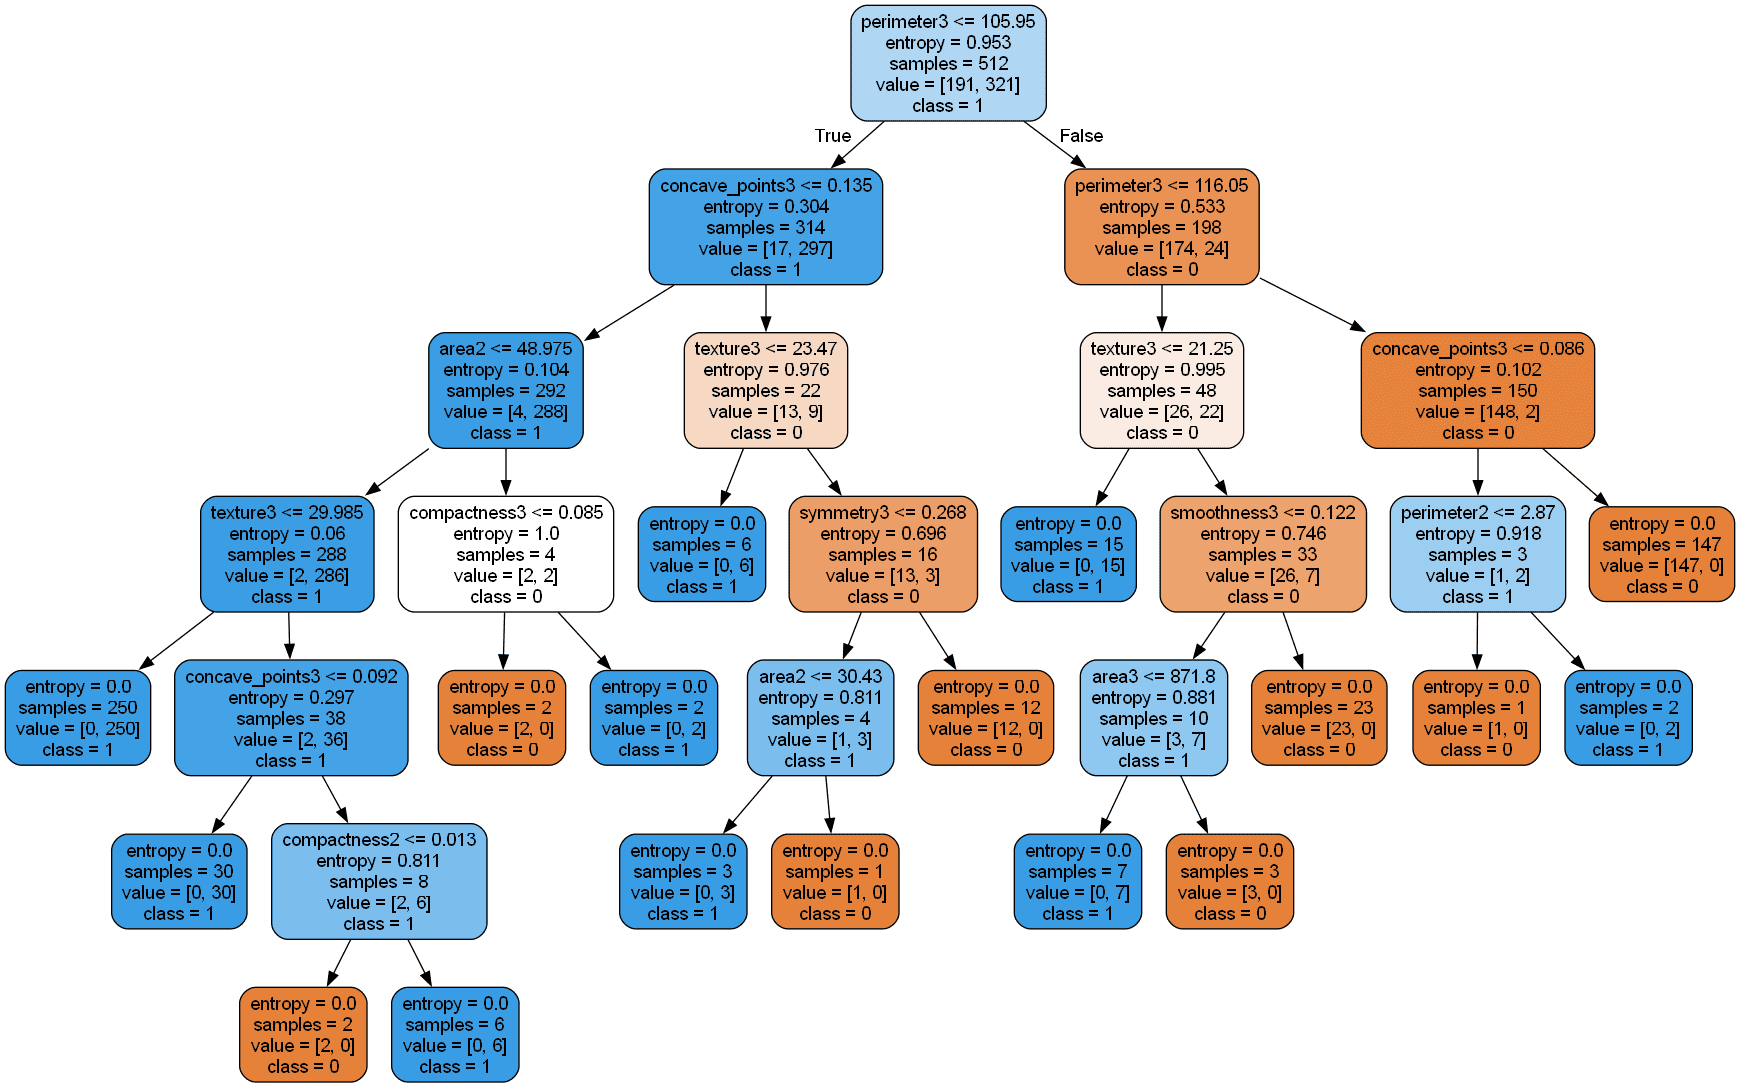
\includegraphics[width=0.65\textwidth]{imgs/dt-mini/dt__breast_cancer__90_vs_10.png}
	\caption{Breast Cancer: decision tree for 90/10 split.}\label{fig:bc-dt-90-10}
\end{figure}

\clearpage
\subsubsection*{Evaluating the decision tree classifiers}
\begin{figure}[H]
	\centering
	\begin{subfigure}{0.45\textwidth}
		\centering
		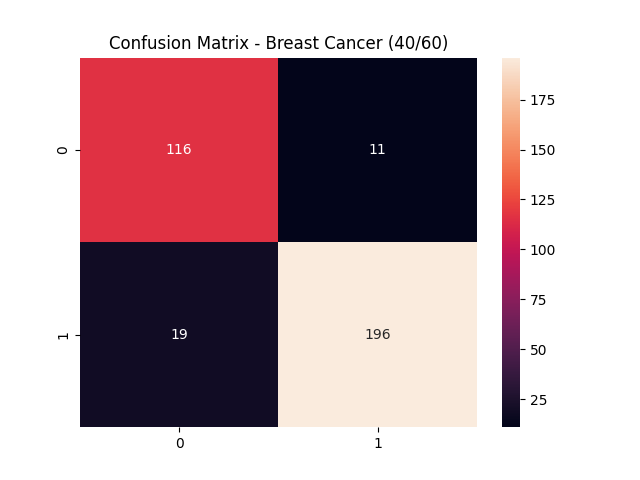
\includegraphics[width=\textwidth]{imgs/confusion_mat/confusion_mat__breast_cancer__40_vs_60.png}
		\caption{Breast Cancer: confusion matrix (40/60 split).}\label{fig:bc-cm-40-60}
	\end{subfigure}
	\hfill
	\begin{subfigure}{0.45\textwidth}
		\centering
		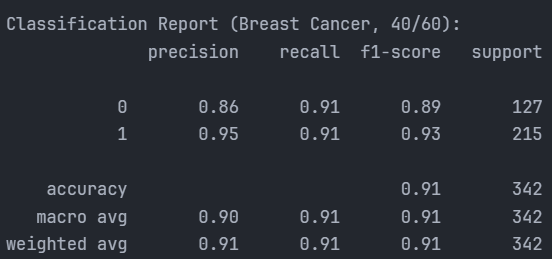
\includegraphics[width=\textwidth]{imgs/confusion_mat/class_rp__breast_cancer__40_vs_60.png}
		\caption{Breast Cancer: Classification Report (40/60 split).}\label{fig:bc-cr-40-60}
	\end{subfigure}

	\caption{Classification Report and Confusion Matrix (40/60 split)}\label{fig:bc-eval-40-60}
\end{figure}
\begin{figure}[H]
	\centering
	\begin{subfigure}{0.45\textwidth}
		\centering
		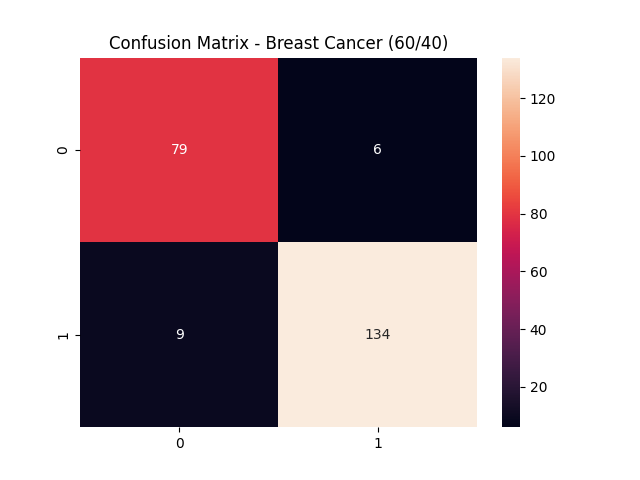
\includegraphics[width=\textwidth]{imgs/confusion_mat/confusion_mat__breast_cancer__60_vs_40.png}
		\caption{Breast Cancer: confusion matrix (60/40 split).}\label{fig:bc-cm-60-40}
	\end{subfigure}
	\hfill
	\begin{subfigure}{0.45\textwidth}
		\centering
		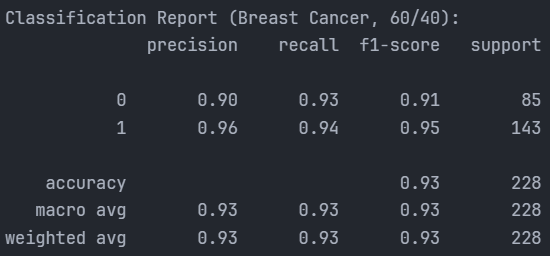
\includegraphics[width=\textwidth]{imgs/confusion_mat/class_rp__breast_cancer__60_vs_40.png}
		\caption{Breast Cancer: Classification Report (60/40 split).}\label{fig:bc-cr-60-40}
	\end{subfigure}

	\caption{Classification Report and Confusion Matrix (60/40 split)}\label{fig:bc-eval-60-40}
\end{figure}
\begin{figure}[H]
	\centering
	\begin{subfigure}{0.45\textwidth}
		\centering
		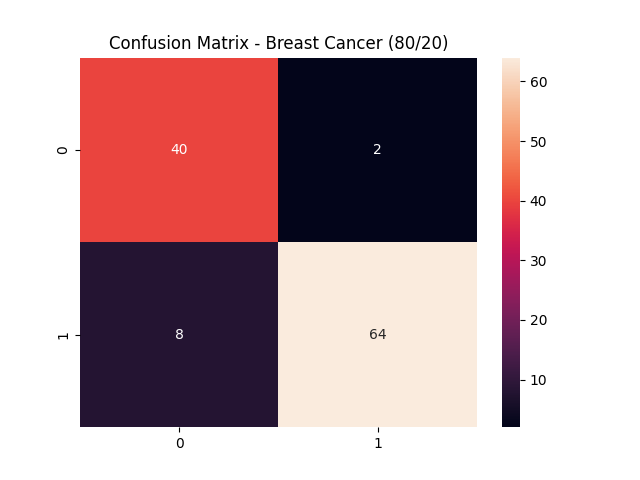
\includegraphics[width=\textwidth]{imgs/confusion_mat/confusion_mat__breast_cancer__80_vs_20.png}
		\caption{Breast Cancer: confusion matrix (80/20 split).}\label{fig:bc-cm-80-20}
	\end{subfigure}
	\hfill
	\begin{subfigure}{0.45\textwidth}
		\centering
		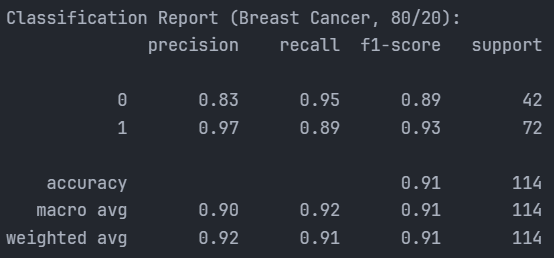
\includegraphics[width=\textwidth]{imgs/confusion_mat/class_rp__breast_cancer__80_vs_20.png}
		\caption{Breast Cancer: Classification Report (80/20 split).}\label{fig:bc-cr-80-20}
	\end{subfigure}

	\caption{Classification Report and Confusion Matrix (80/20 split)}\label{fig:bc-eval-80-20}
\end{figure}
\begin{figure}[H]
	\centering
	\begin{subfigure}{0.45\textwidth}
		\centering
		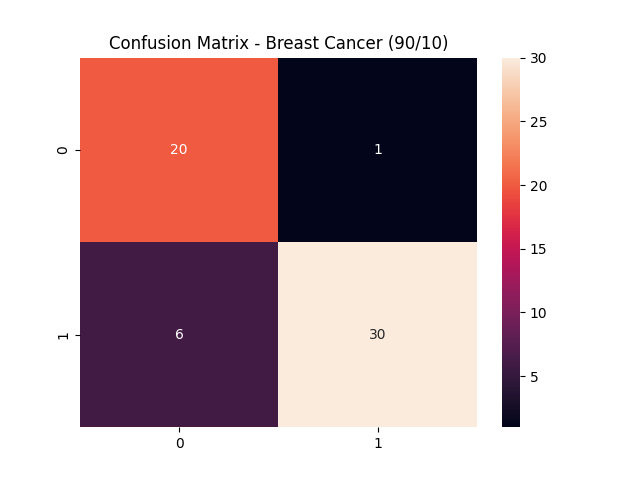
\includegraphics[width=\textwidth]{imgs/confusion_mat/confusion_mat__breast_cancer__90_vs_10.png}
		\caption{Breast Cancer: confusion matrix (90/10 split).}\label{fig:bc-cm-90-10}
	\end{subfigure}
	\hfill
	\begin{subfigure}{0.45\textwidth}
		\centering
		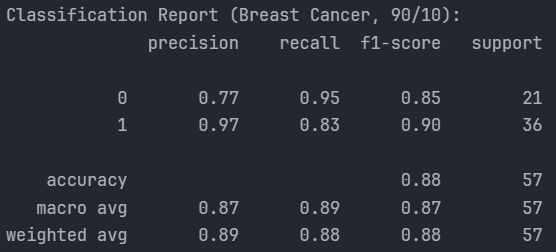
\includegraphics[width=\textwidth]{imgs/confusion_mat/class_rp__breast_cancer__90_vs_10.png}
		\caption{Breast Cancer: Classification Report (90/10 split).}\label{fig:bc-cr-90-10}
	\end{subfigure}

	\caption{Classification Report and Confusion Matrix (90/10 split)}\label{fig:bc-eval-90-10}
\end{figure}
\begin{flushleft}
	Insights into performance of these decision tree classifiers:
	\begin{itemize}
		\item sth
		      \begin{itemize}
			      \item sth
		      \end{itemize}
	\end{itemize}
\end{flushleft}

\clearpage
\subsubsection*{Decision Tree Classifier with Different Depths}
\begin{figure}[H]
	\centering
	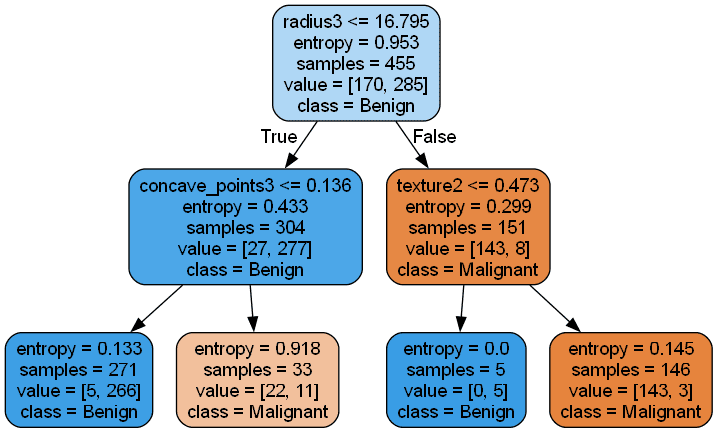
\includegraphics[width=0.65\textwidth]{imgs/dt-mini/dt__breast_cancer__80_vs_20__2.png}
	\caption{Breast Cancer: decision tree with \texttt{max\_depth}=2 (80/20 split).}\label{fig:bc-dt-depth-2}
\end{figure}

\begin{figure}[H]
	\centering
	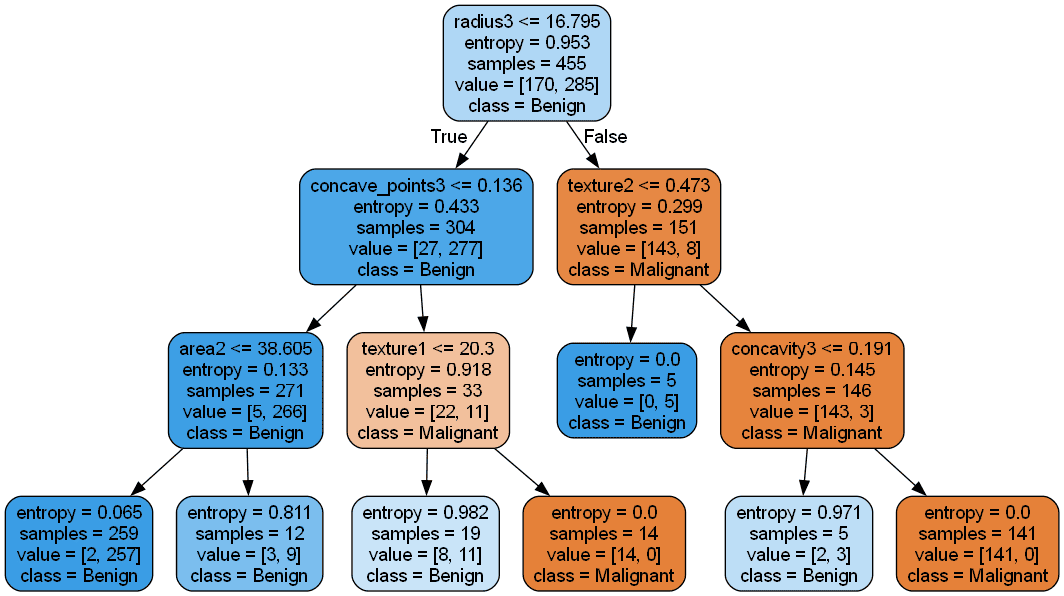
\includegraphics[width=0.65\textwidth]{imgs/dt-mini/dt__breast_cancer__80_vs_20__3.png}
	\caption{Breast Cancer: decision tree with \texttt{max\_depth}=3 (80/20 split).}\label{fig:bc-dt-depth-3}
\end{figure}

\begin{figure}[H]
	\centering
	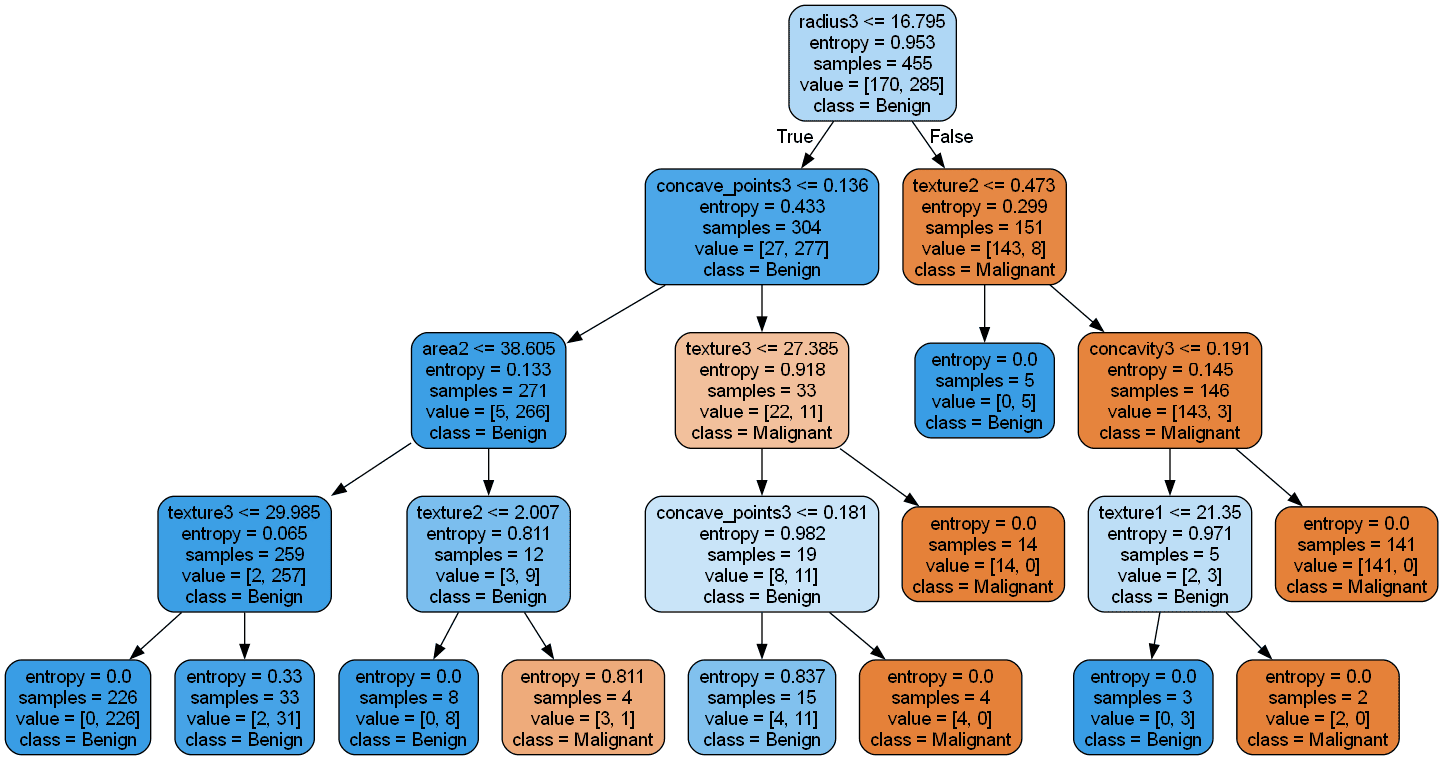
\includegraphics[width=0.65\textwidth]{imgs/dt-mini/dt__breast_cancer__80_vs_20__4.png}
	\caption{Breast Cancer: decision tree with \texttt{max\_depth}=4 (80/20 split).}\label{fig:bc-dt-depth-4}
\end{figure}

\begin{figure}[H]
	\centering
	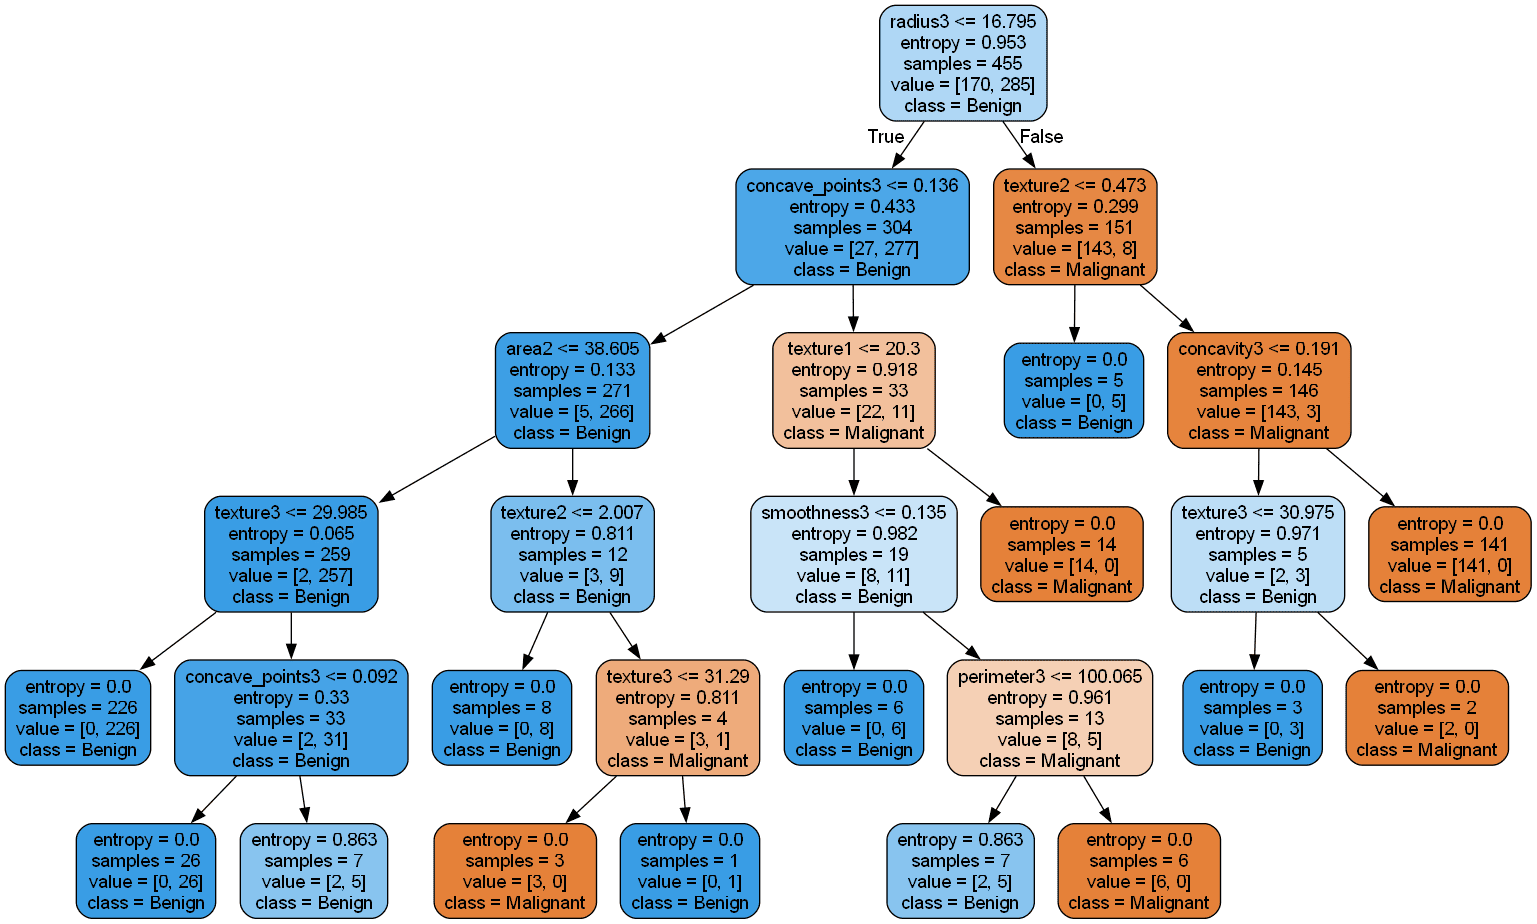
\includegraphics[width=0.65\textwidth]{imgs/dt-mini/dt__breast_cancer__80_vs_20__5.png}
	\caption{Breast Cancer: decision tree with \texttt{max\_depth}=5 (80/20 split).}\label{fig:bc-dt-depth-5}
\end{figure}

\begin{figure}[H]
	\centering
	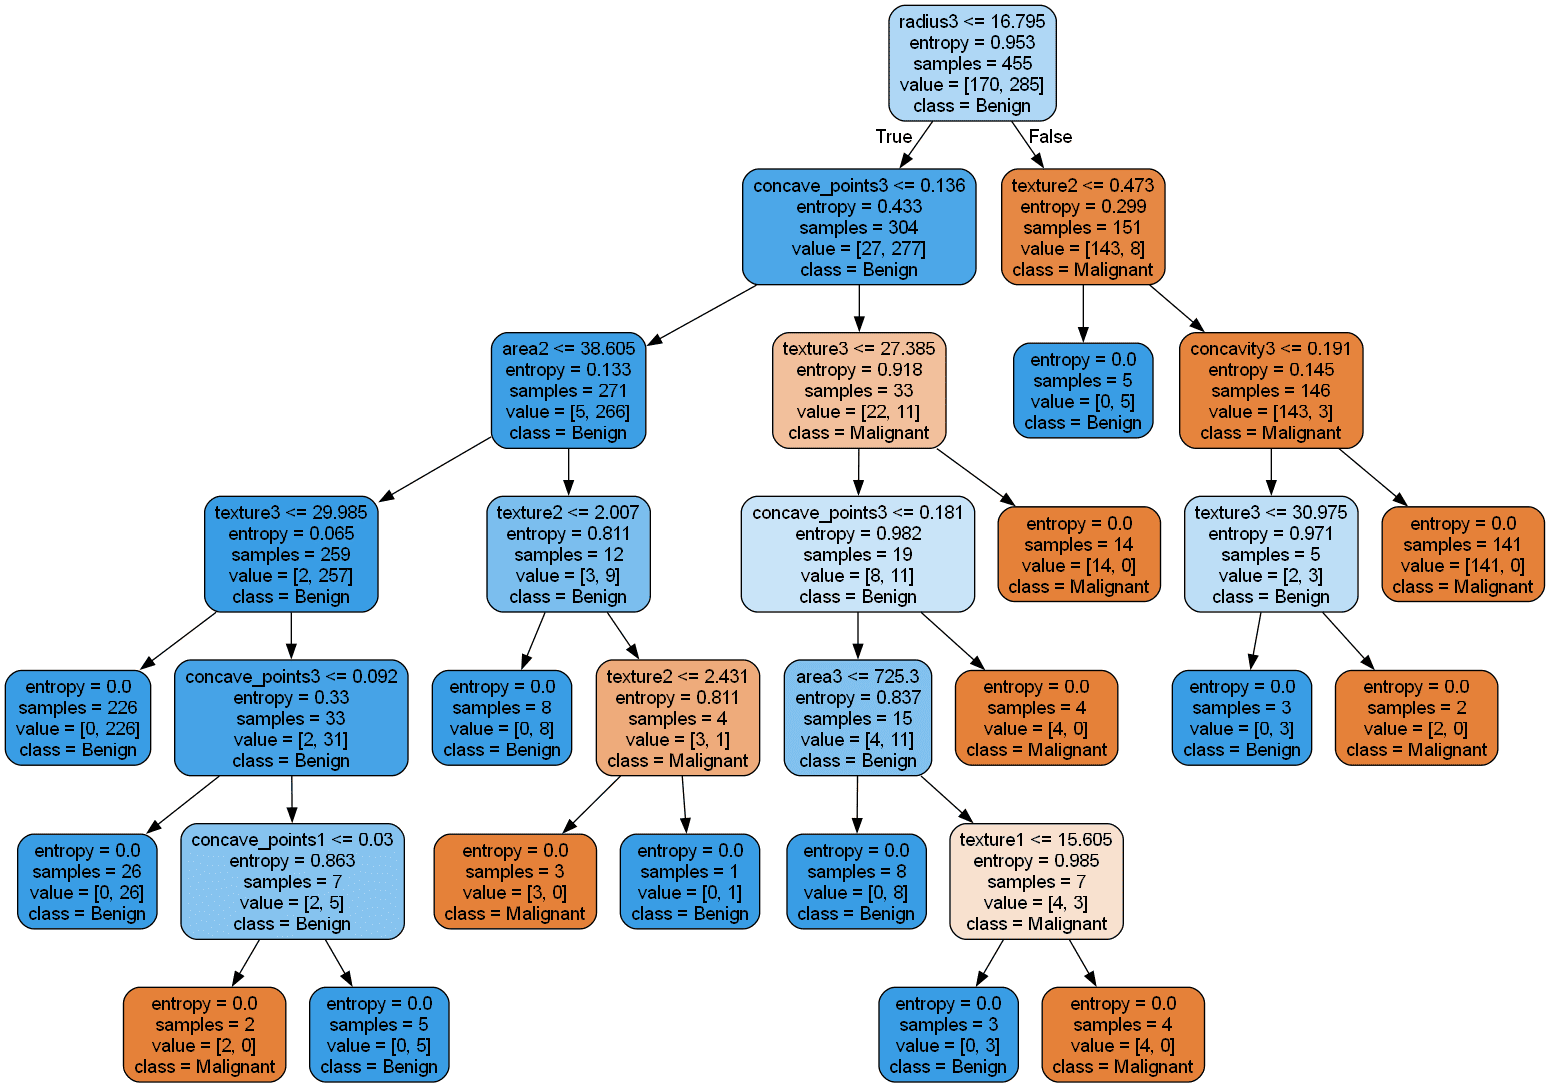
\includegraphics[width=0.65\textwidth]{imgs/dt-mini/dt__breast_cancer__80_vs_20__6.png}
	\caption{Breast Cancer: decision tree with \texttt{max\_depth}=6 (80/20 split).}\label{fig:bc-dt-depth-6}
\end{figure}

\begin{figure}[H]
	\centering
	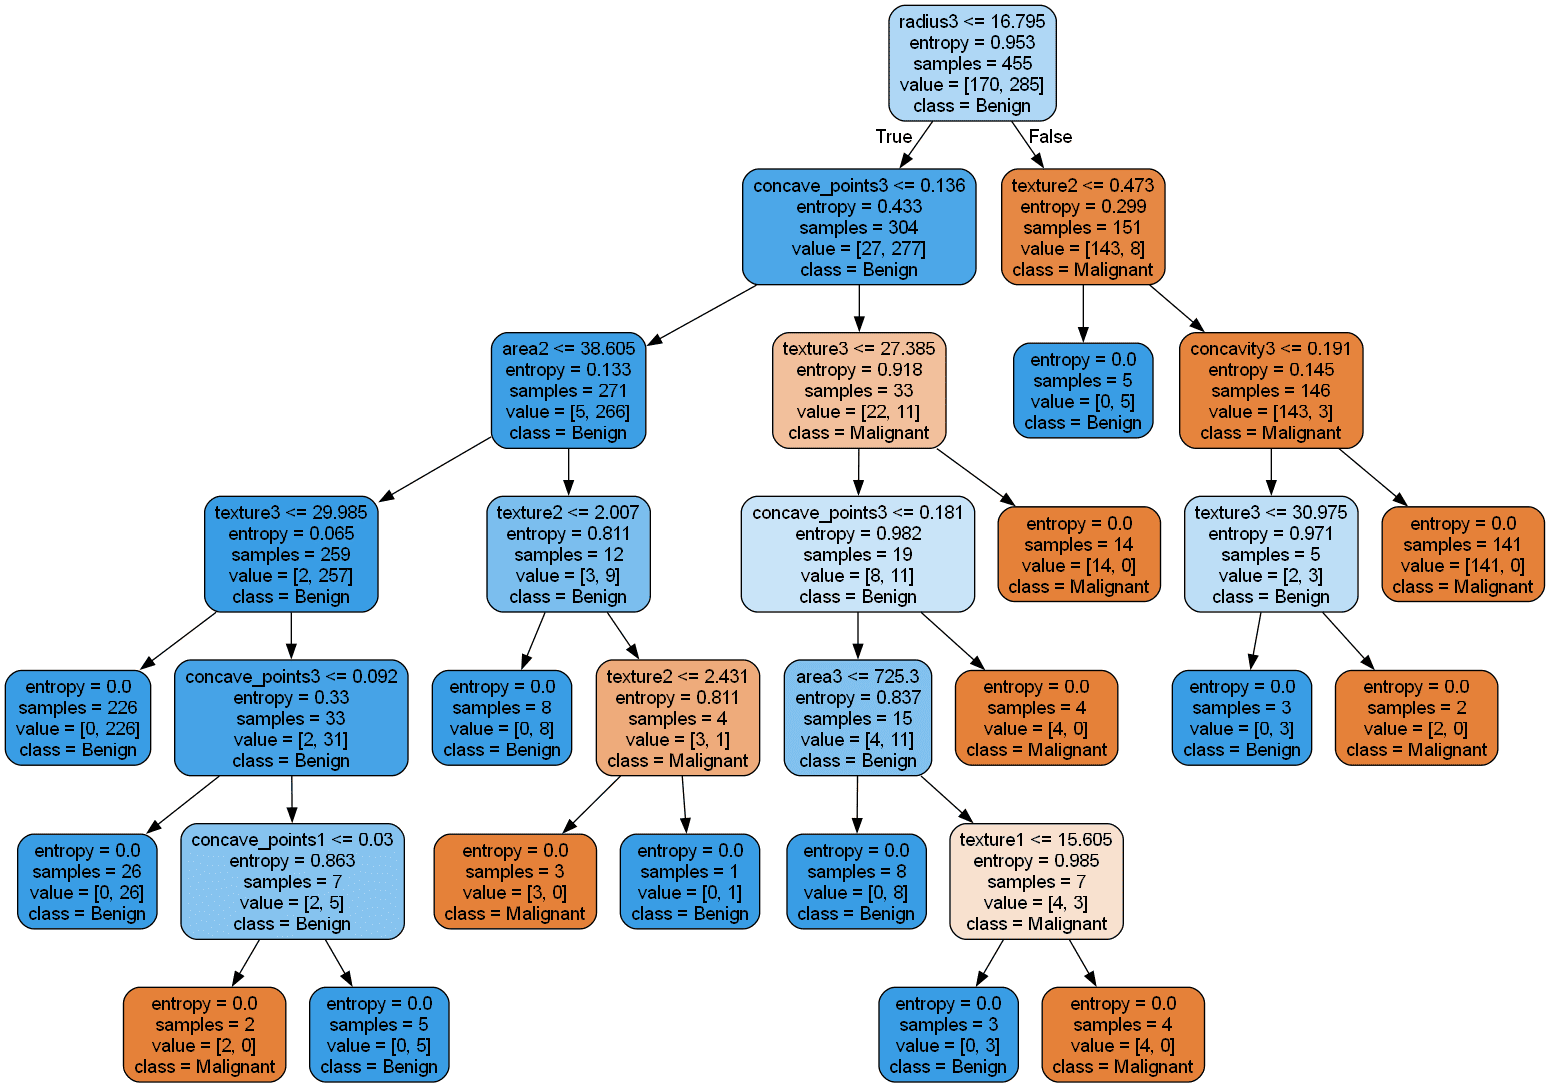
\includegraphics[width=0.65\textwidth]{imgs/dt-mini/dt__breast_cancer__80_vs_20__7.png}
	\caption{Breast Cancer: decision tree with \texttt{max\_depth}=7 (80/20 split).}\label{fig:bc-dt-depth-7}
\end{figure}

\begin{figure}[H]
	\centering
	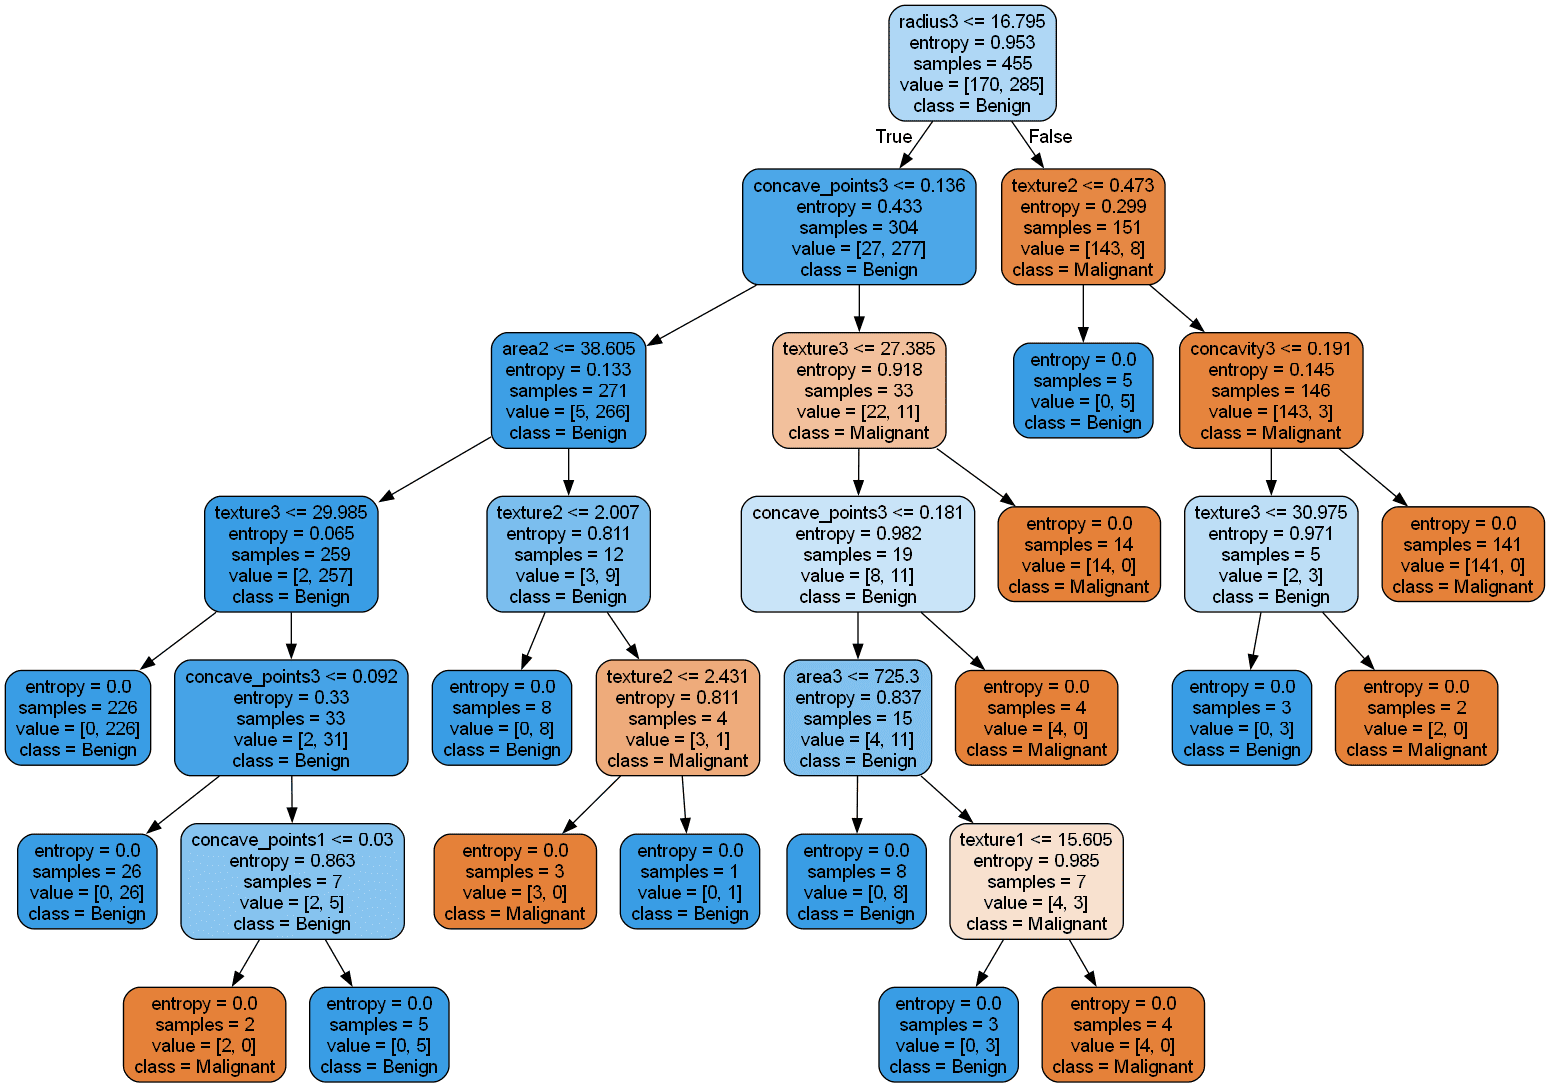
\includegraphics[width=0.65\textwidth]{imgs/dt-mini/dt__breast_cancer__80_vs_20__None.png}
	\caption{Breast Cancer: decision tree with \texttt{max\_depth}=None (80/20 split).}\label{fig:bc-dt-depth-none}
\end{figure}

\begin{figure}[H]
	\centering
	\begin{subfigure}{0.45\textwidth}
		\centering
		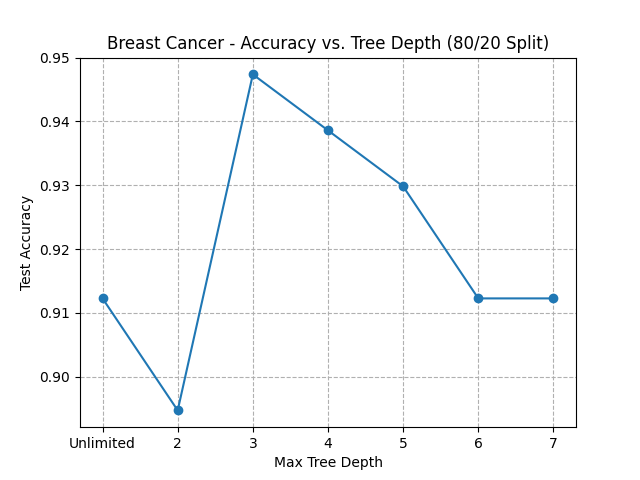
\includegraphics[width=\textwidth]{imgs/accuracy_vs_depth_breast_cancer.png}
	\end{subfigure}
	\hfill
	\begin{subfigure}{0.45\textwidth}
		\centering
		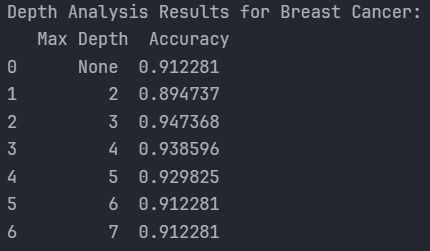
\includegraphics[width=\textwidth]{imgs/accuracy_vs_depth_breast_cancer__analysis.png}
	\end{subfigure}
\end{figure}

\clearpage
\subsubsection*{Insights}
\begin{itemize}
	\item sth
	      \begin{itemize}
		      \item sth
	      \end{itemize}
\end{itemize}

%================ Wine Quality =================%
\clearpage
\subsection{Wine Quality Dataset}
\begin{itemize}
	\item \textbf{Description:} 4,898 samples; original scores 0–10 grouped into Low (0–4), Standard (5–6), High (7–10).
	\item \textbf{Preprocessing:} label encoding, stratified splits at 40/60, 60/40, 80/20, 90/10.
\end{itemize}

\begin{figure}[H]
	\centering
	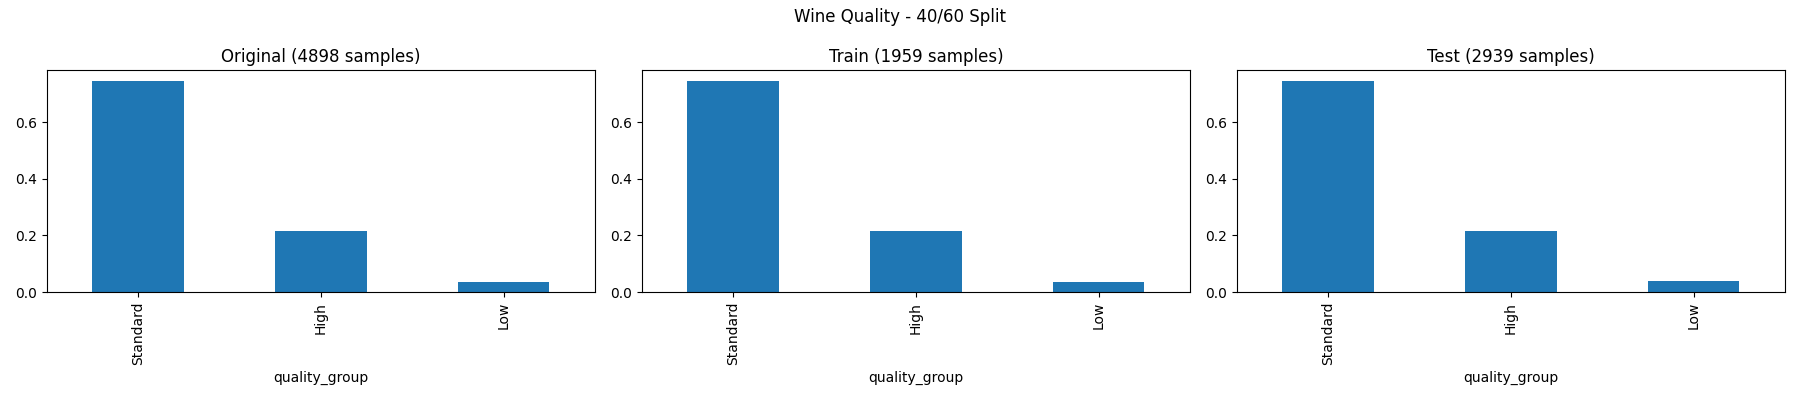
\includegraphics[width=0.6\textwidth]{imgs/class_dist/class_dist__wine_quality__40_vs_60.png}
	\caption{Wine Quality: class distribution (40/60 split).}\label{fig:wq-cd-40-60}
\end{figure}

\begin{figure}[H]
	\centering
	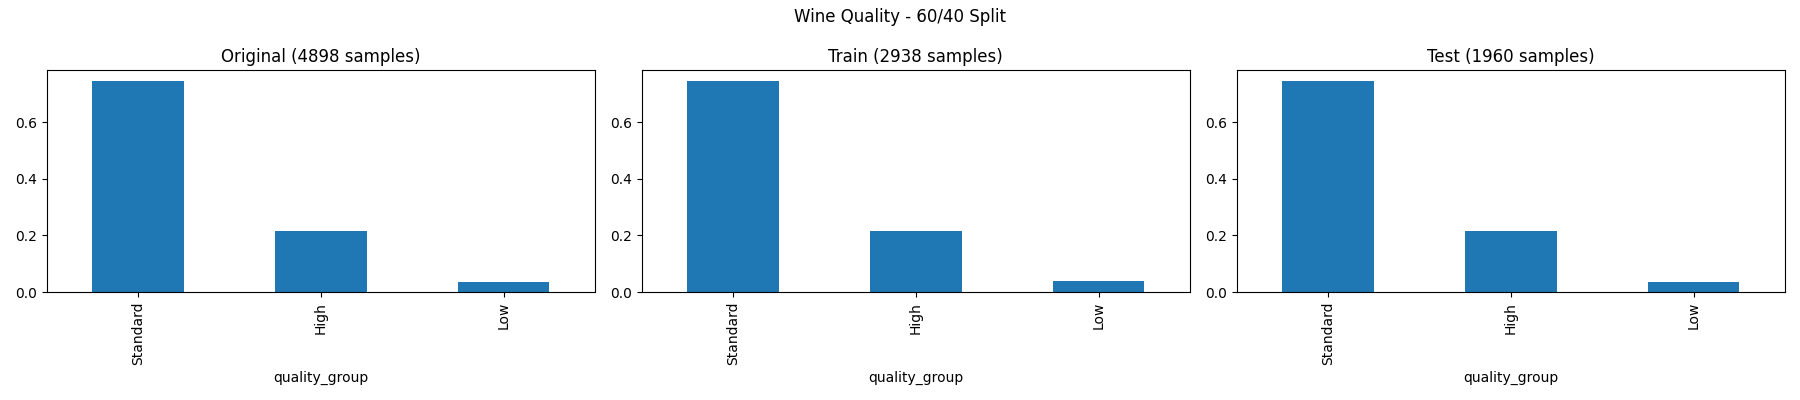
\includegraphics[width=0.6\textwidth]{imgs/class_dist/class_dist__wine_quality__60_vs_40.png}
	\caption{Wine Quality: class distribution (60/40 split).}\label{fig:wq-cd-60-40}
\end{figure}

\begin{figure}[H]
	\centering
	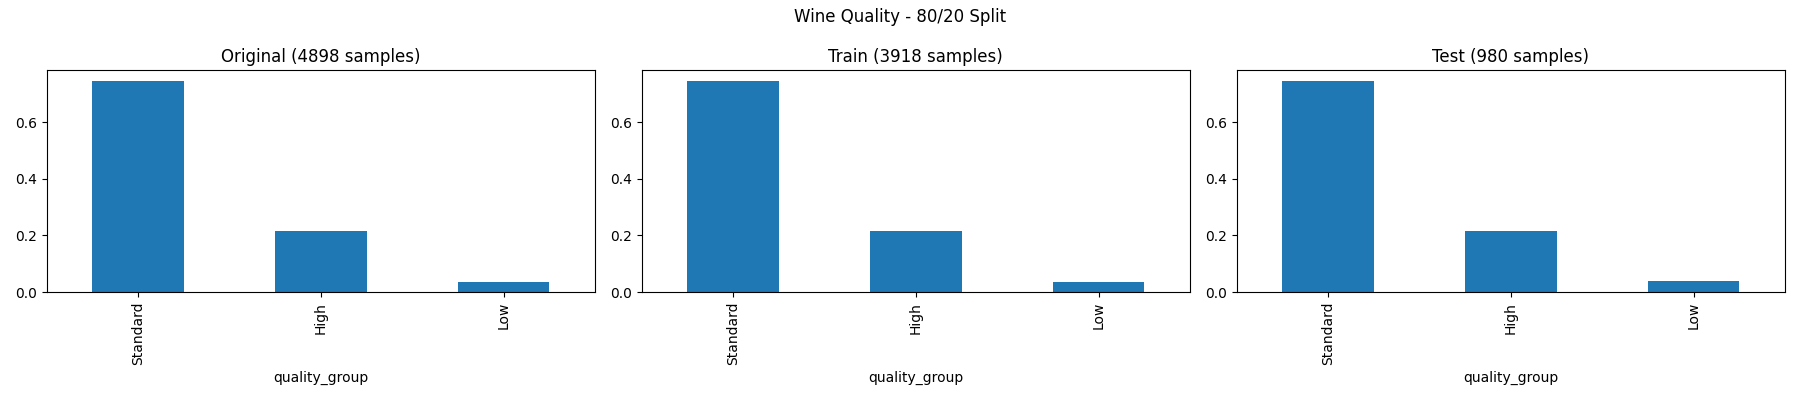
\includegraphics[width=0.6\textwidth]{imgs/class_dist/class_dist__wine_quality__80_vs_20.png}
	\caption{Wine Quality: class distribution (80/20 split).}\label{fig:wq-cd-80-20}
\end{figure}

\begin{figure}[H]
	\centering
	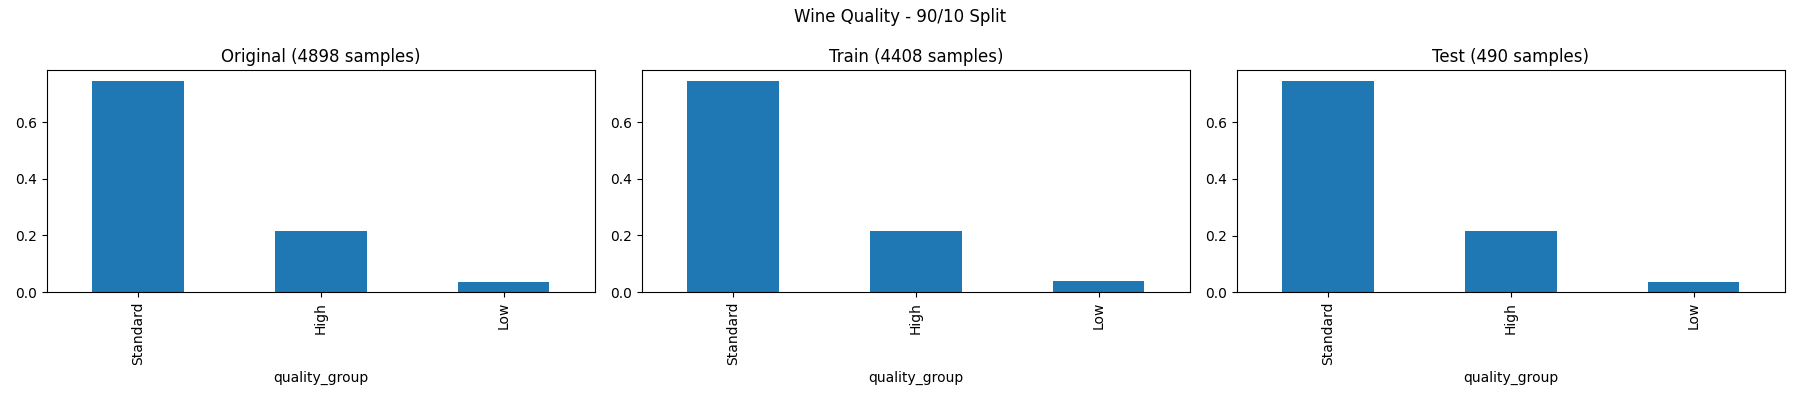
\includegraphics[width=0.6\textwidth]{imgs/class_dist/class_dist__wine_quality__90_vs_10.png}
	\caption{Wine Quality: class distribution (90/10 split).}\label{fig:wq-cd-90-10}
\end{figure}

\begin{figure}[H]
	\centering
	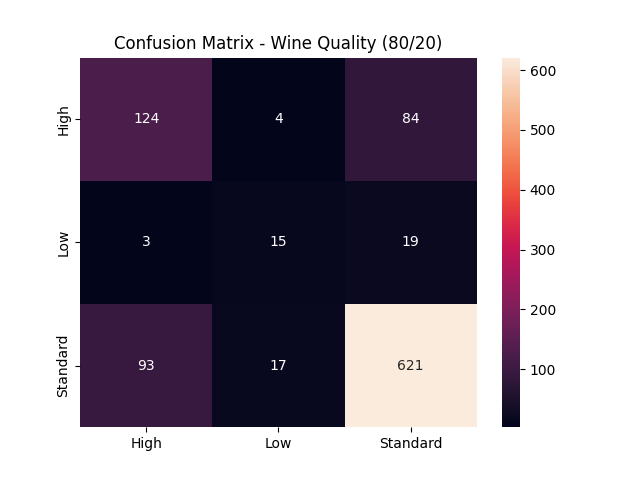
\includegraphics[width=0.6\textwidth]{imgs/confusion_mat/confusion_mat__wine_quality__80_vs_20.png}
	\caption{Wine Quality: confusion matrix (80/20 split).}\label{fig:wq-cm-80-20}
\end{figure}

% \begin{figure}[H]
% 	\centering
% 	\includegraphics[width=0.8\textwidth]{imgs/dt-mini/dt__wine_quality__80_vs_20.png}
% 	\caption{Wine Quality: decision tree (base) for 80/20 split.}\label{fig:wq-dt-base}
% \end{figure}

\begin{figure}[H]
	\centering
	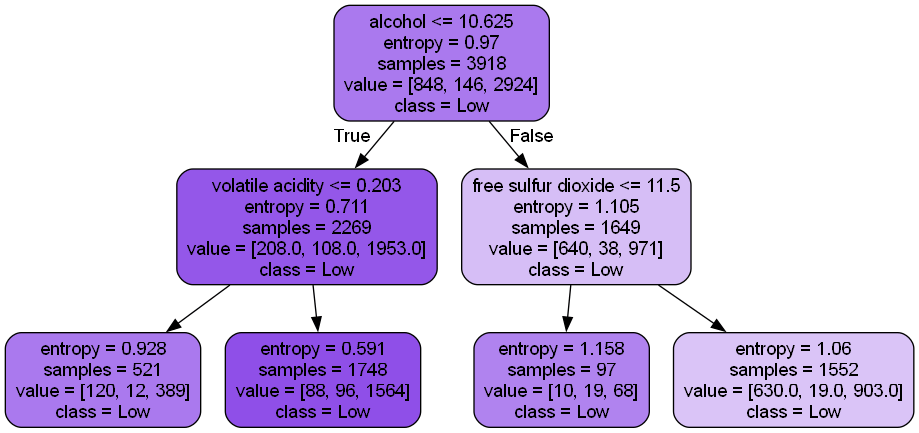
\includegraphics[width=0.8\textwidth]{imgs/dt-mini/dt__wine_quality__80_vs_20__2.png}
	\caption{Wine Quality: decision tree with \texttt{max\_depth}=2 (80/20 split).}\label{fig:wq-dt-depth-2}
\end{figure}

\begin{figure}[H]
	\centering
	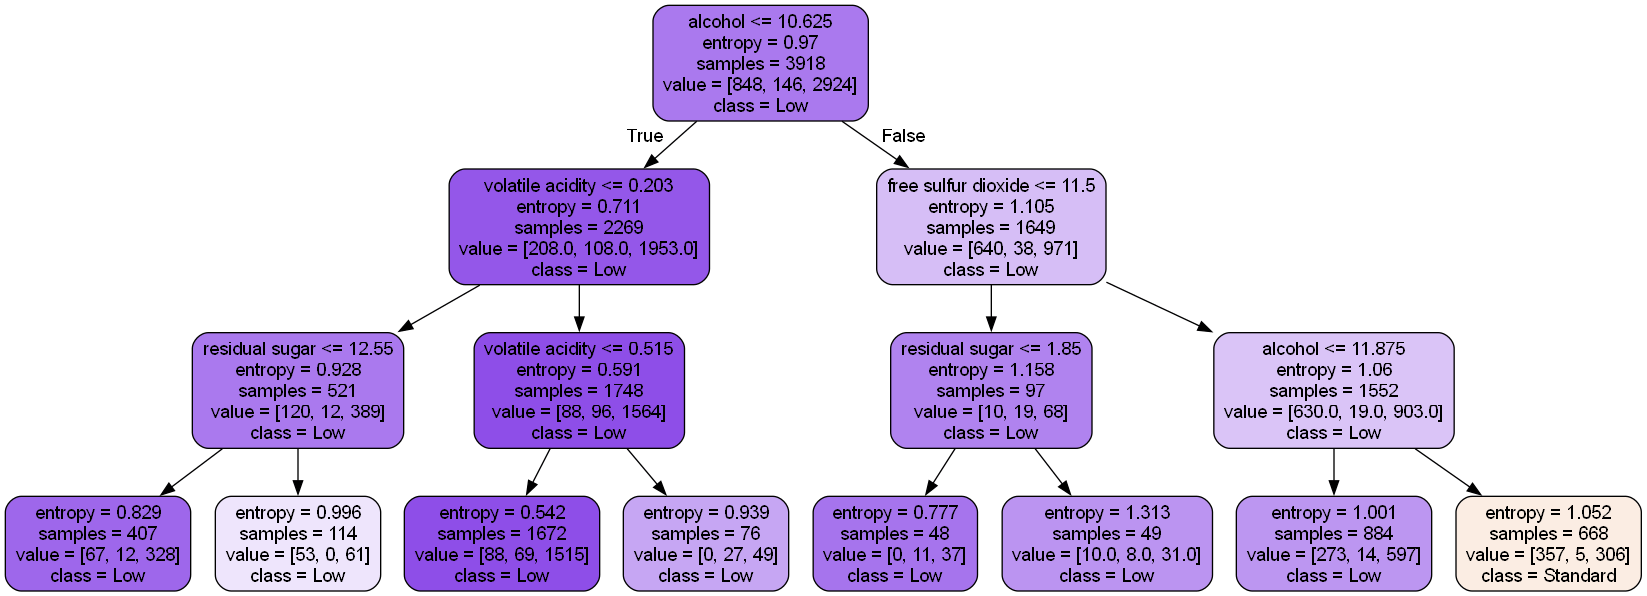
\includegraphics[width=0.8\textwidth]{imgs/dt-mini/dt__wine_quality__80_vs_20__3.png}
	\caption{Wine Quality: decision tree with \texttt{max\_depth}=3 (80/20 split).}\label{fig:wq-dt-depth-3}
\end{figure}

\begin{figure}[H]
	\centering
	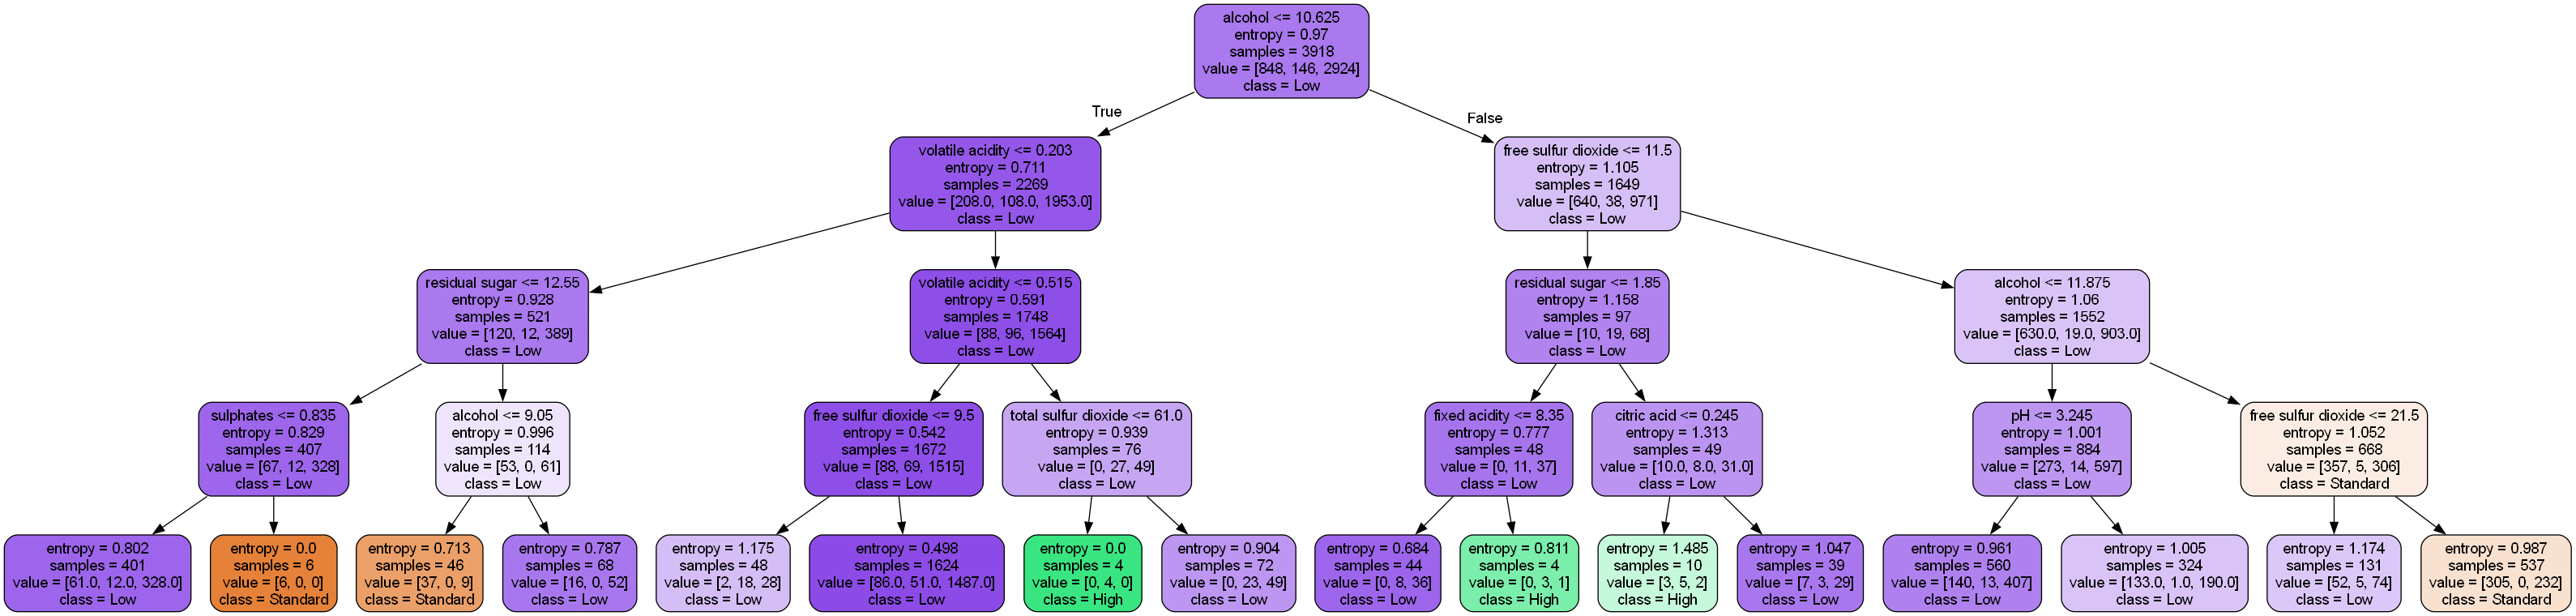
\includegraphics[width=0.8\textwidth]{imgs/dt-mini/dt__wine_quality__80_vs_20__4.png}
	\caption{Wine Quality: decision tree with \texttt{max\_depth}=4 (80/20 split).}\label{fig:wq-dt-depth-4}
\end{figure}

\begin{figure}[H]
	\centering
	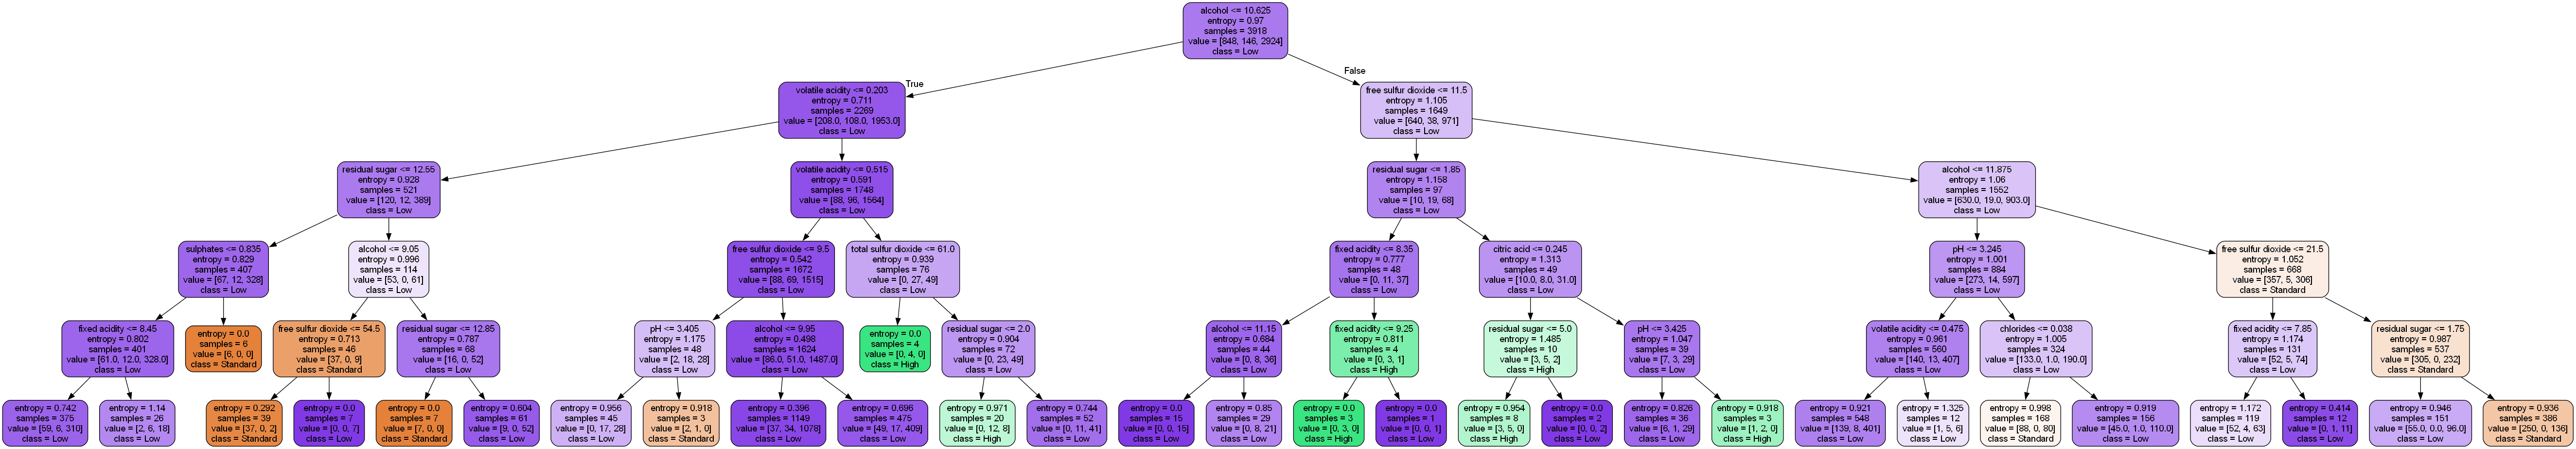
\includegraphics[width=0.8\textwidth]{imgs/dt-mini/dt__wine_quality__80_vs_20__5.png}
	\caption{Wine Quality: decision tree with \texttt{max\_depth}=5 (80/20 split).}\label{fig:wq-dt-depth-5}
\end{figure}

\begin{figure}[H]
	\centering
	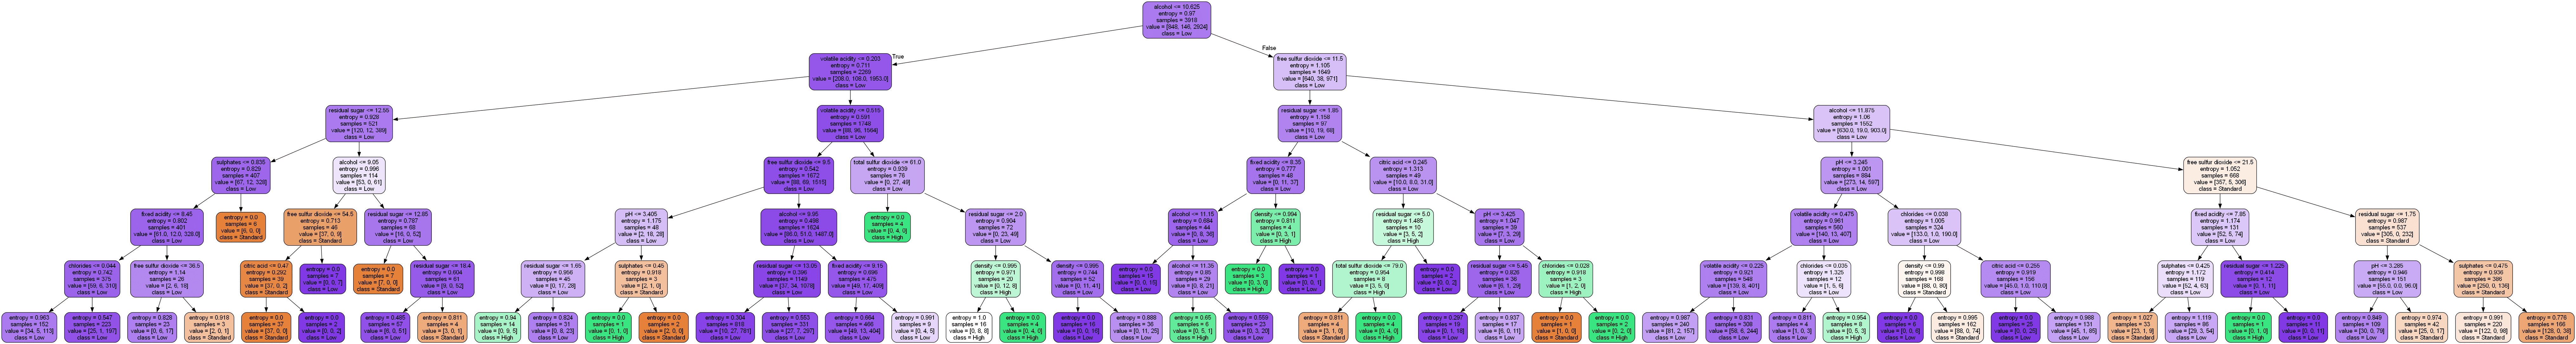
\includegraphics[width=0.8\textwidth]{imgs/dt-mini/dt__wine_quality__80_vs_20__6.png}
	\caption{Wine Quality: decision tree with \texttt{max\_depth}=6 (80/20 split).}\label{fig:wq-dt-depth-6}
\end{figure}

\begin{figure}[H]
	\centering
	
\includegraphics[width=0.8\textwidth]{imgs/dt-mini/dt__wine_quality__80_vs_20__7.png}
	\caption{Wine Quality: decision tree with \texttt{max\_depth}=7 (80/20 split).}\label{fig:wq-dt-depth-7}
\end{figure}

% \begin{figure}[H]
% 	\centering
% 	\includegraphics[width=0.8\textwidth]{imgs/dt-mini/dt__wine_quality__80_vs_20__None.png}
% 	\caption{Wine Quality: decision tree with \texttt{max\_depth}=None (80/20 split).}\label{fig:wq-dt-depth-none}
% \end{figure}

%================ Car Evaluation =================%
\clearpage
\subsection{Car Evaluation Dataset}
\begin{itemize}
	\item \textbf{Description:} 1,728 samples; 4 classes (\texttt{unacc}, \texttt{acc}, \texttt{good}, \texttt{vgood}), 6 categorical features.
	\item \textbf{Preprocessing:} label encoding, stratified splits at 40/60, 60/40, 80/20, 90/10.
\end{itemize}

\begin{figure}[H]
	\centering
	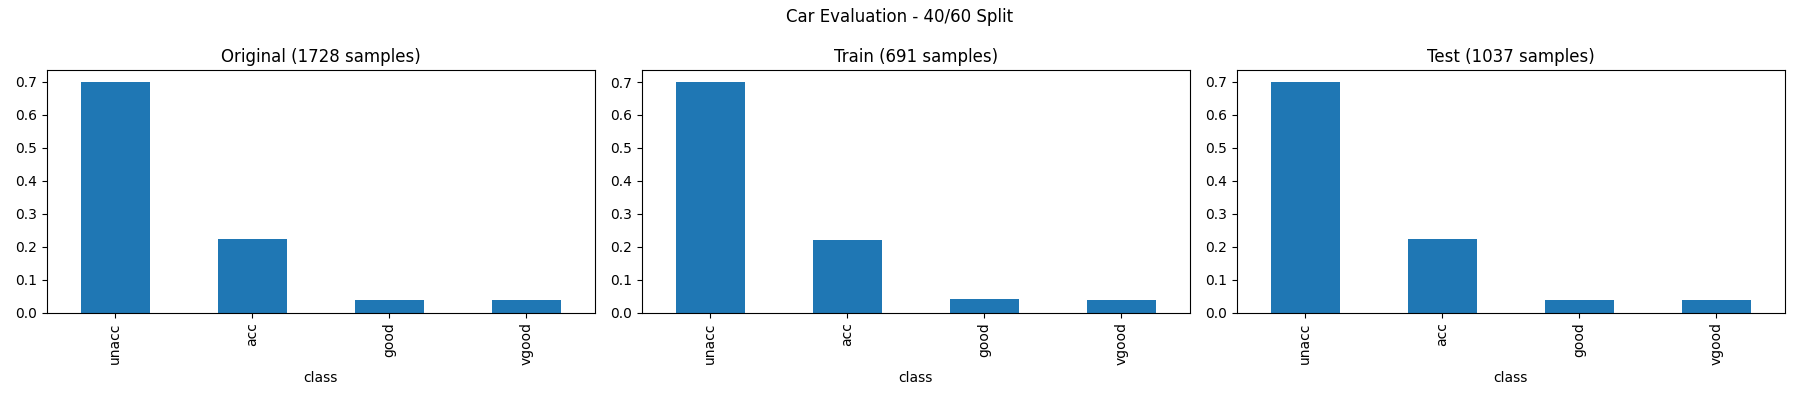
\includegraphics[width=0.6\textwidth]{imgs/class_dist/class_dist__car_evaluation__40_vs_60.png}
	\caption{Car Evaluation: class distribution (40/60 split).}\label{fig:ce-cd-40-60}
\end{figure}

\begin{figure}[H]
	\centering
	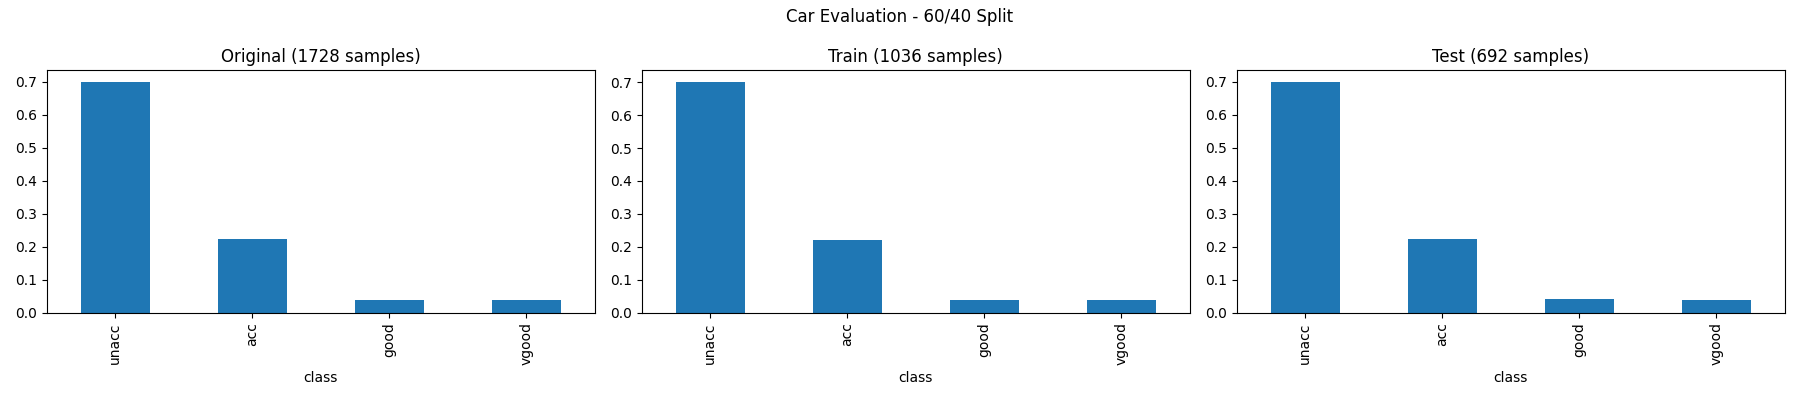
\includegraphics[width=0.6\textwidth]{imgs/class_dist/class_dist__car_evaluation__60_vs_40.png}
	\caption{Car Evaluation: class distribution (60/40 split).}\label{fig:ce-cd-60-40}
\end{figure}

\begin{figure}[H]
	\centering
	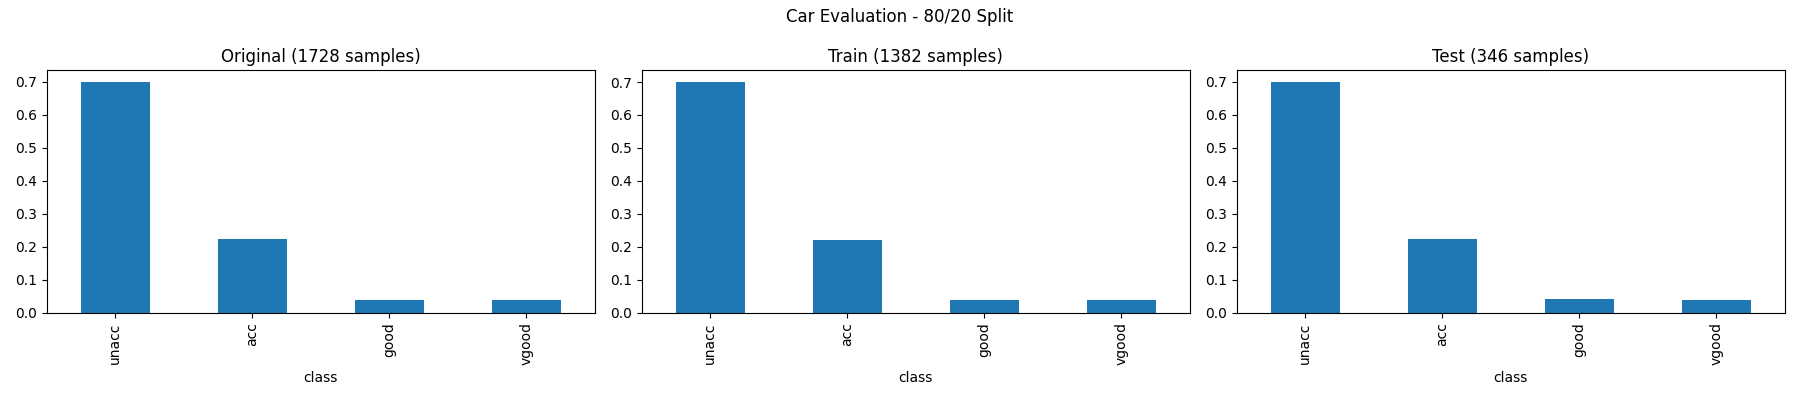
\includegraphics[width=0.6\textwidth]{imgs/class_dist/class_dist__car_evaluation__80_vs_20.png}
	\caption{Car Evaluation: class distribution (80/20 split).}\label{fig:ce-cd-80-20}
\end{figure}

\begin{figure}[H]
	\centering
	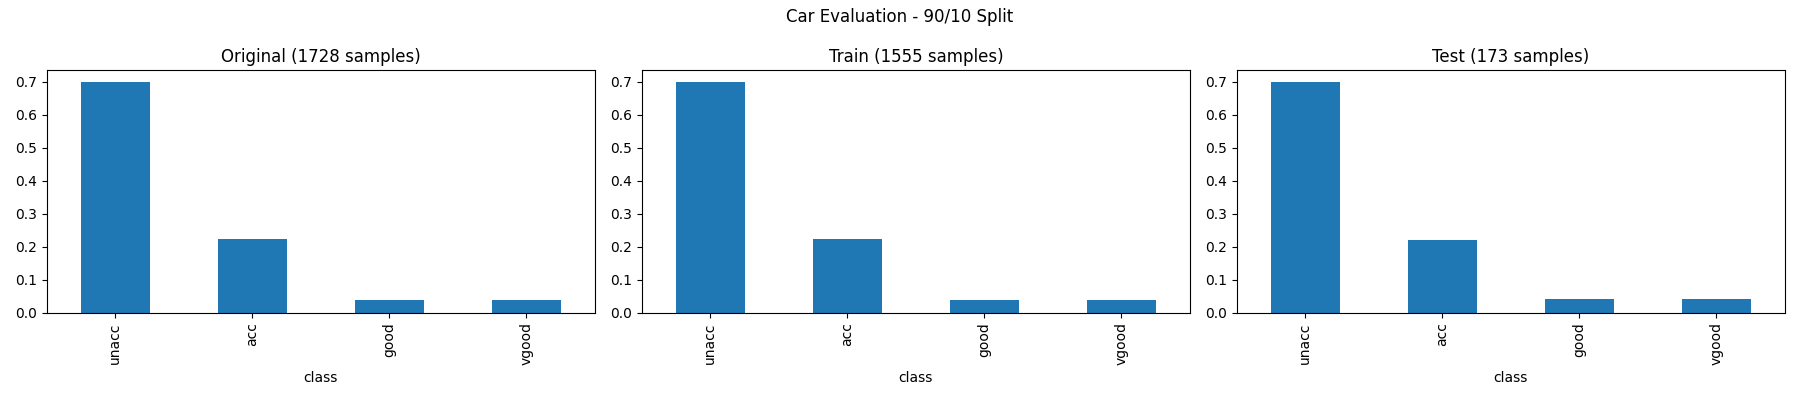
\includegraphics[width=0.6\textwidth]{imgs/class_dist/class_dist__car_evaluation__90_vs_10.png}
	\caption{Car Evaluation: class distribution (90/10 split).}\label{fig:ce-cd-90-10}
\end{figure}

\begin{figure}[H]
	\centering
	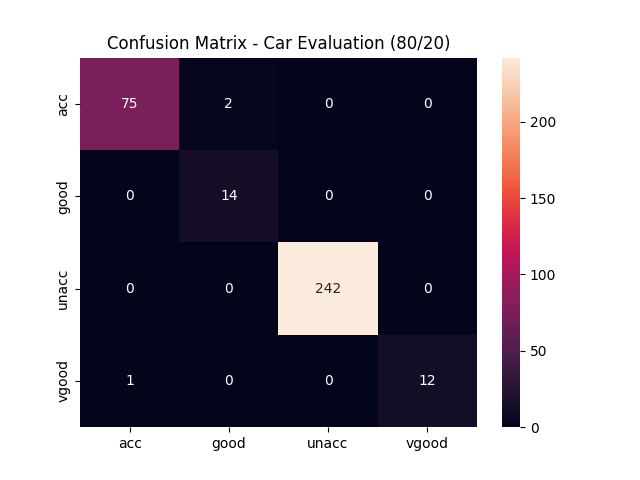
\includegraphics[width=0.6\textwidth]{imgs/confusion_mat/confusion_mat__car_evaluation__80_vs_20.png}
	\caption{Car Evaluation: confusion matrix (80/20 split).}\label{fig:ce-cm-80-20}
\end{figure}

\begin{figure}[H]
	\centering
	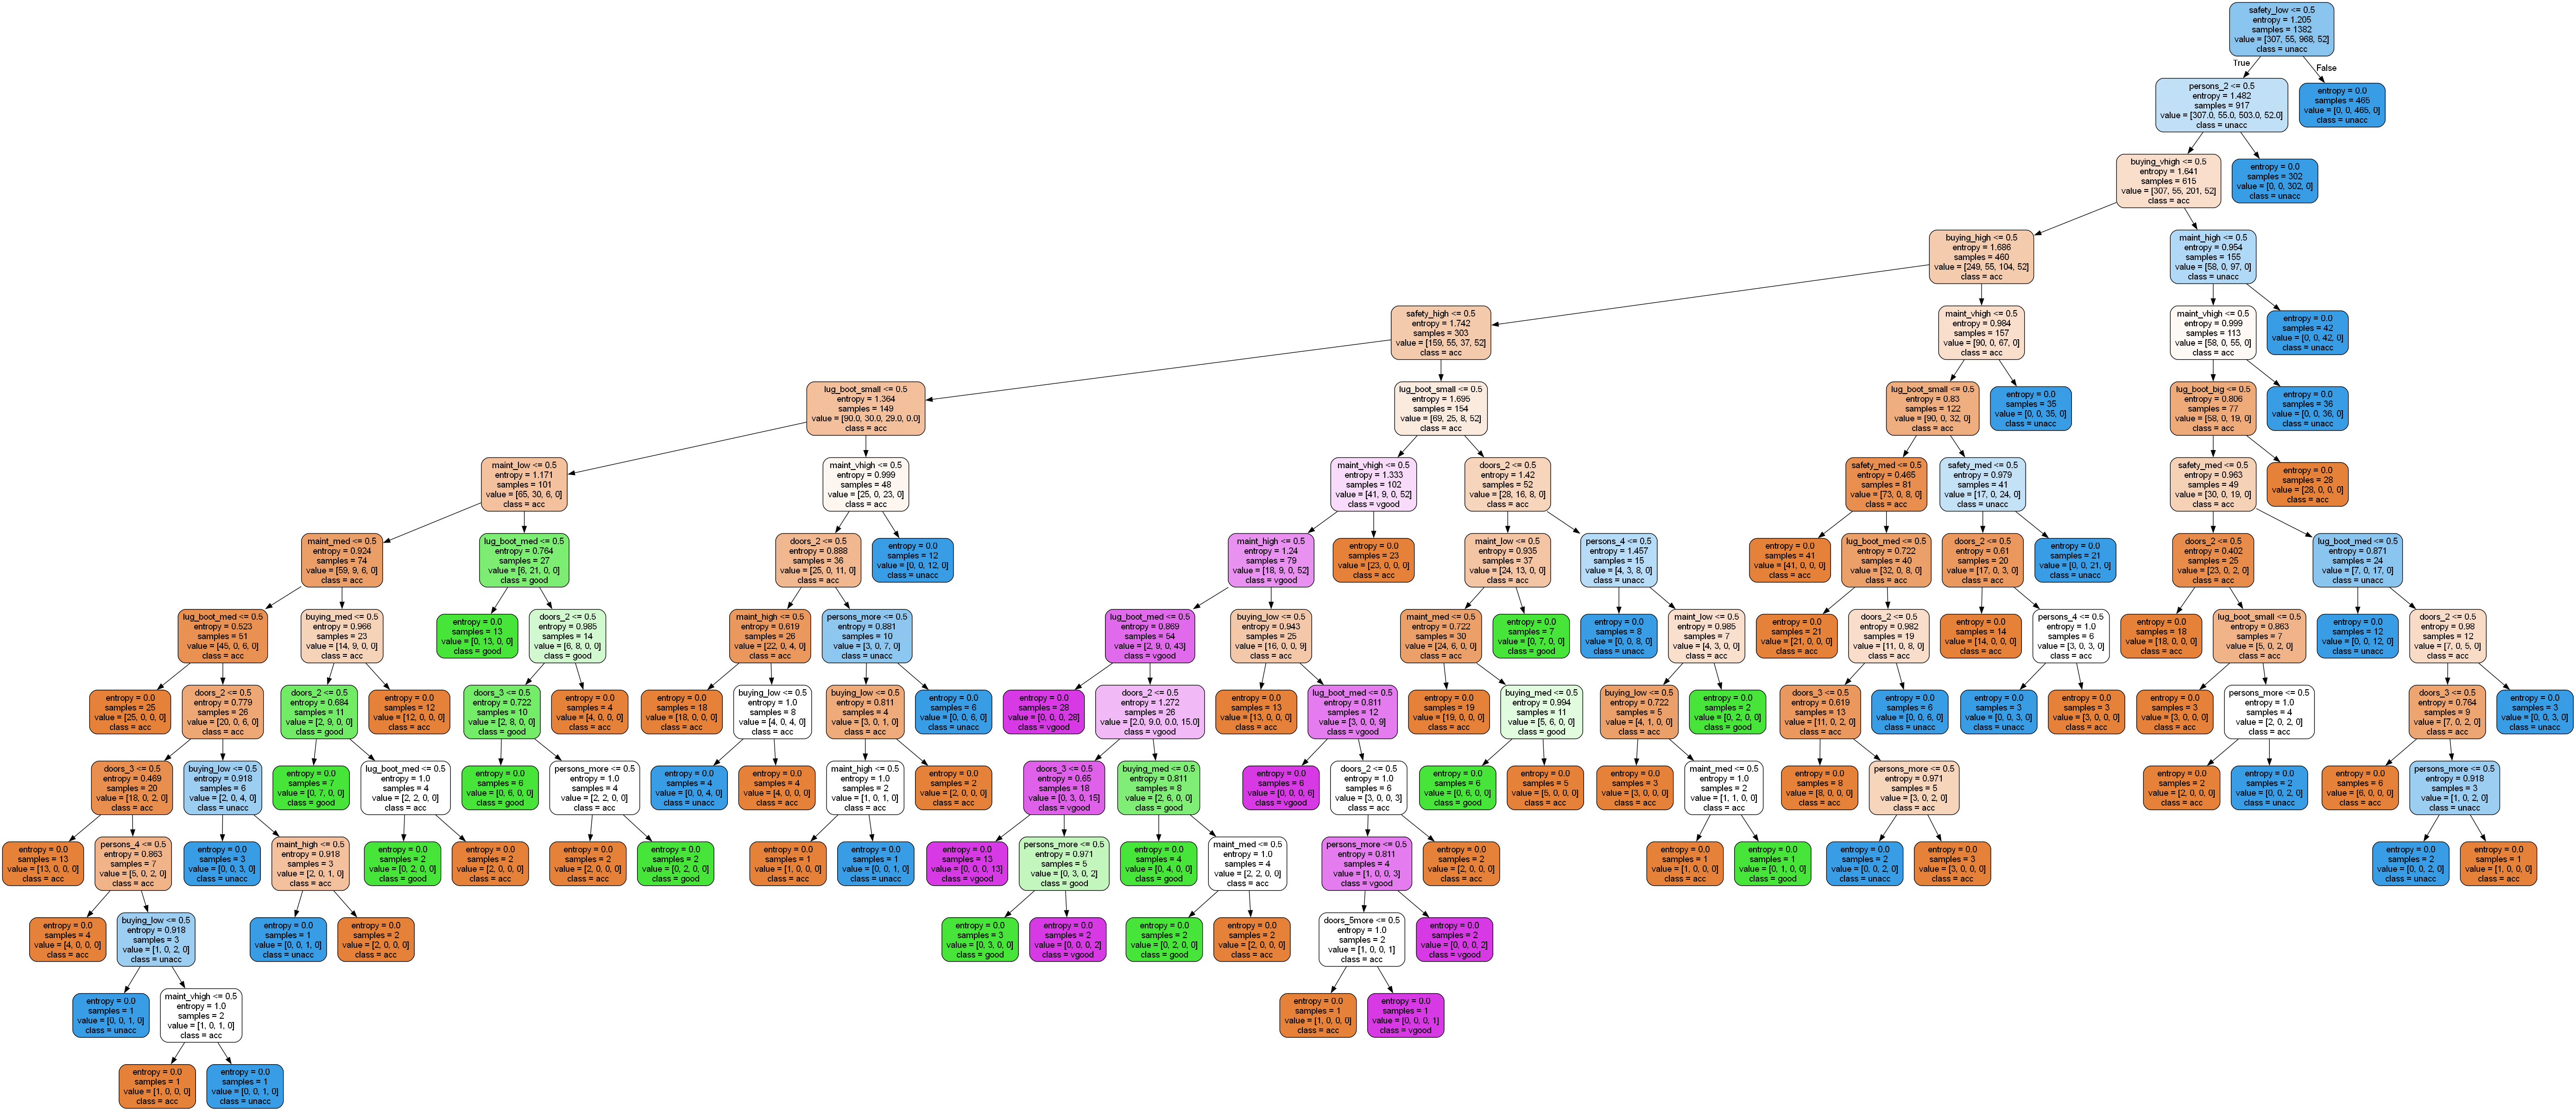
\includegraphics[width=0.8\textwidth]{imgs/dt-mini/dt__car_evaluation__80_vs_20.png}
	\caption{Car Evaluation: decision tree (base) for 80/20 split.}\label{fig:ce-dt-base}
\end{figure}

\begin{figure}[H]
	\centering
	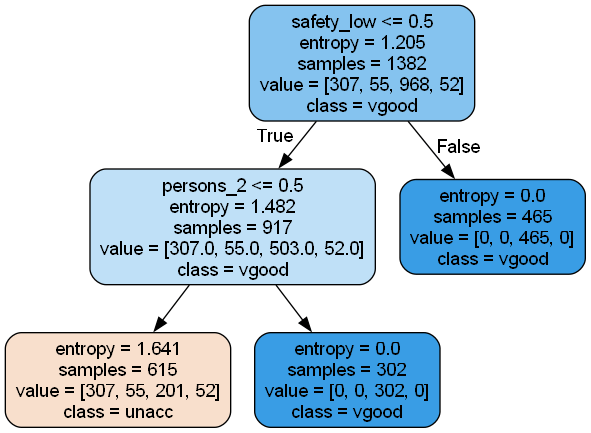
\includegraphics[width=0.8\textwidth]{imgs/dt-mini/dt__car_evaluation__80_vs_20__2.png}
	\caption{Car Evaluation: decision tree with \texttt{max\_depth}=2 (80/20 split).}\label{fig:ce-dt-depth-2}
\end{figure}

\begin{figure}[H]
	\centering
	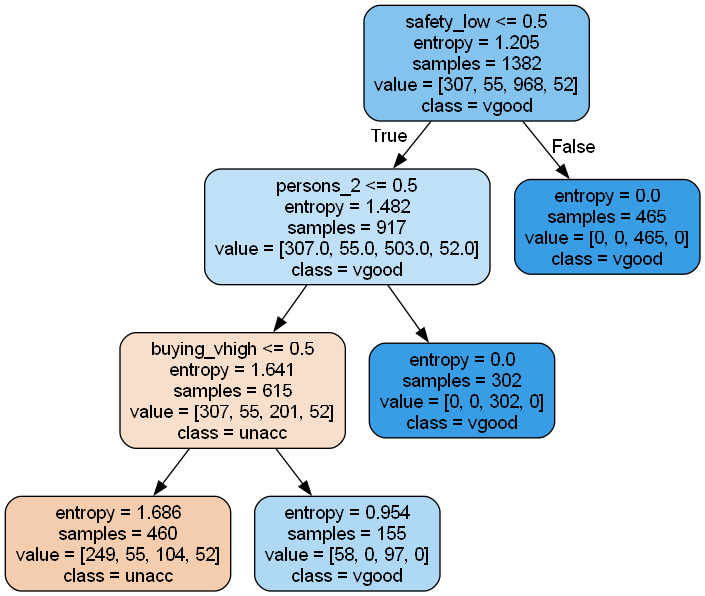
\includegraphics[width=0.8\textwidth]{imgs/dt-mini/dt__car_evaluation__80_vs_20__3.png}
	\caption{Car Evaluation: decision tree with \texttt{max\_depth}=3 (80/20 split).}\label{fig:ce-dt-depth-3}
\end{figure}

\begin{figure}[H]
	\centering
	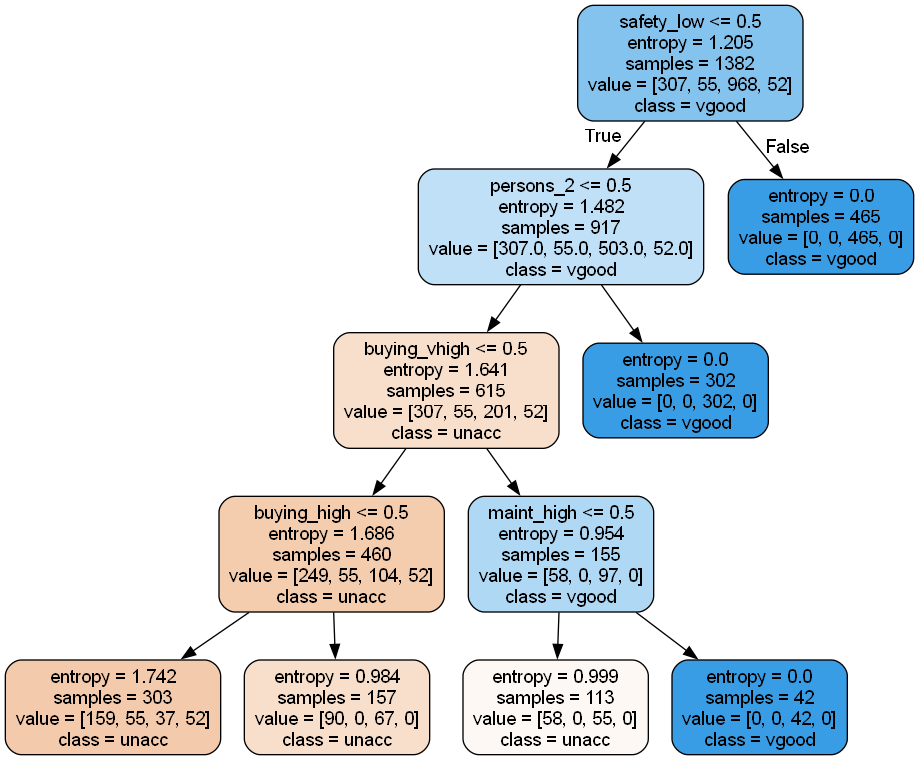
\includegraphics[width=0.8\textwidth]{imgs/dt-mini/dt__car_evaluation__80_vs_20__4.png}
	\caption{Car Evaluation: decision tree with \texttt{max\_depth}=4 (80/20 split).}\label{fig:ce-dt-depth-4}
\end{figure}

\begin{figure}[H]
	\centering
	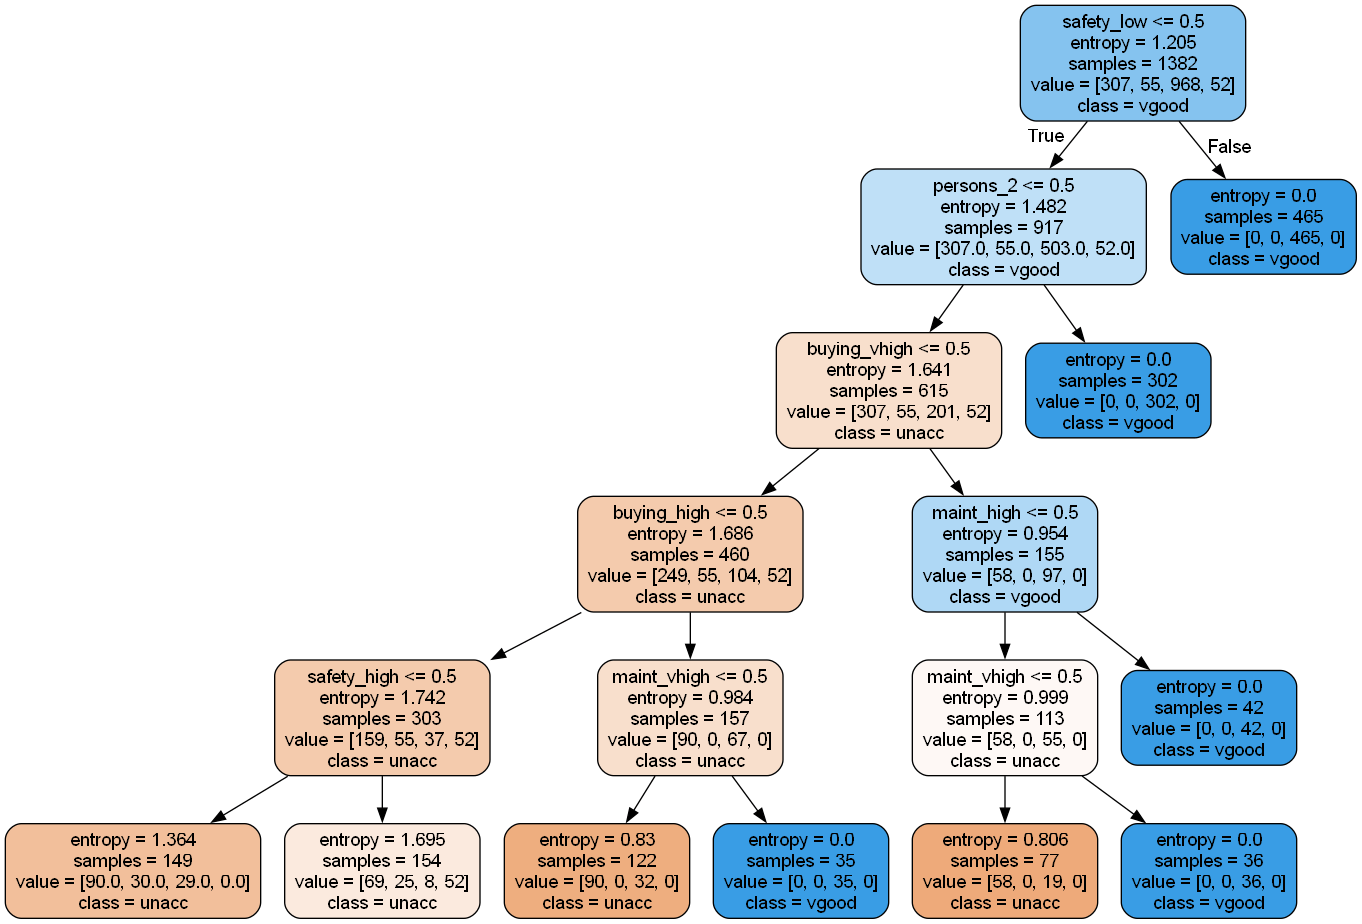
\includegraphics[width=0.8\textwidth]{imgs/dt-mini/dt__car_evaluation__80_vs_20__5.png}
	\caption{Car Evaluation: decision tree with \texttt{max\_depth}=5 (80/20 split).}\label{fig:ce-dt-depth-5}
\end{figure}

\begin{figure}[H]
	\centering
	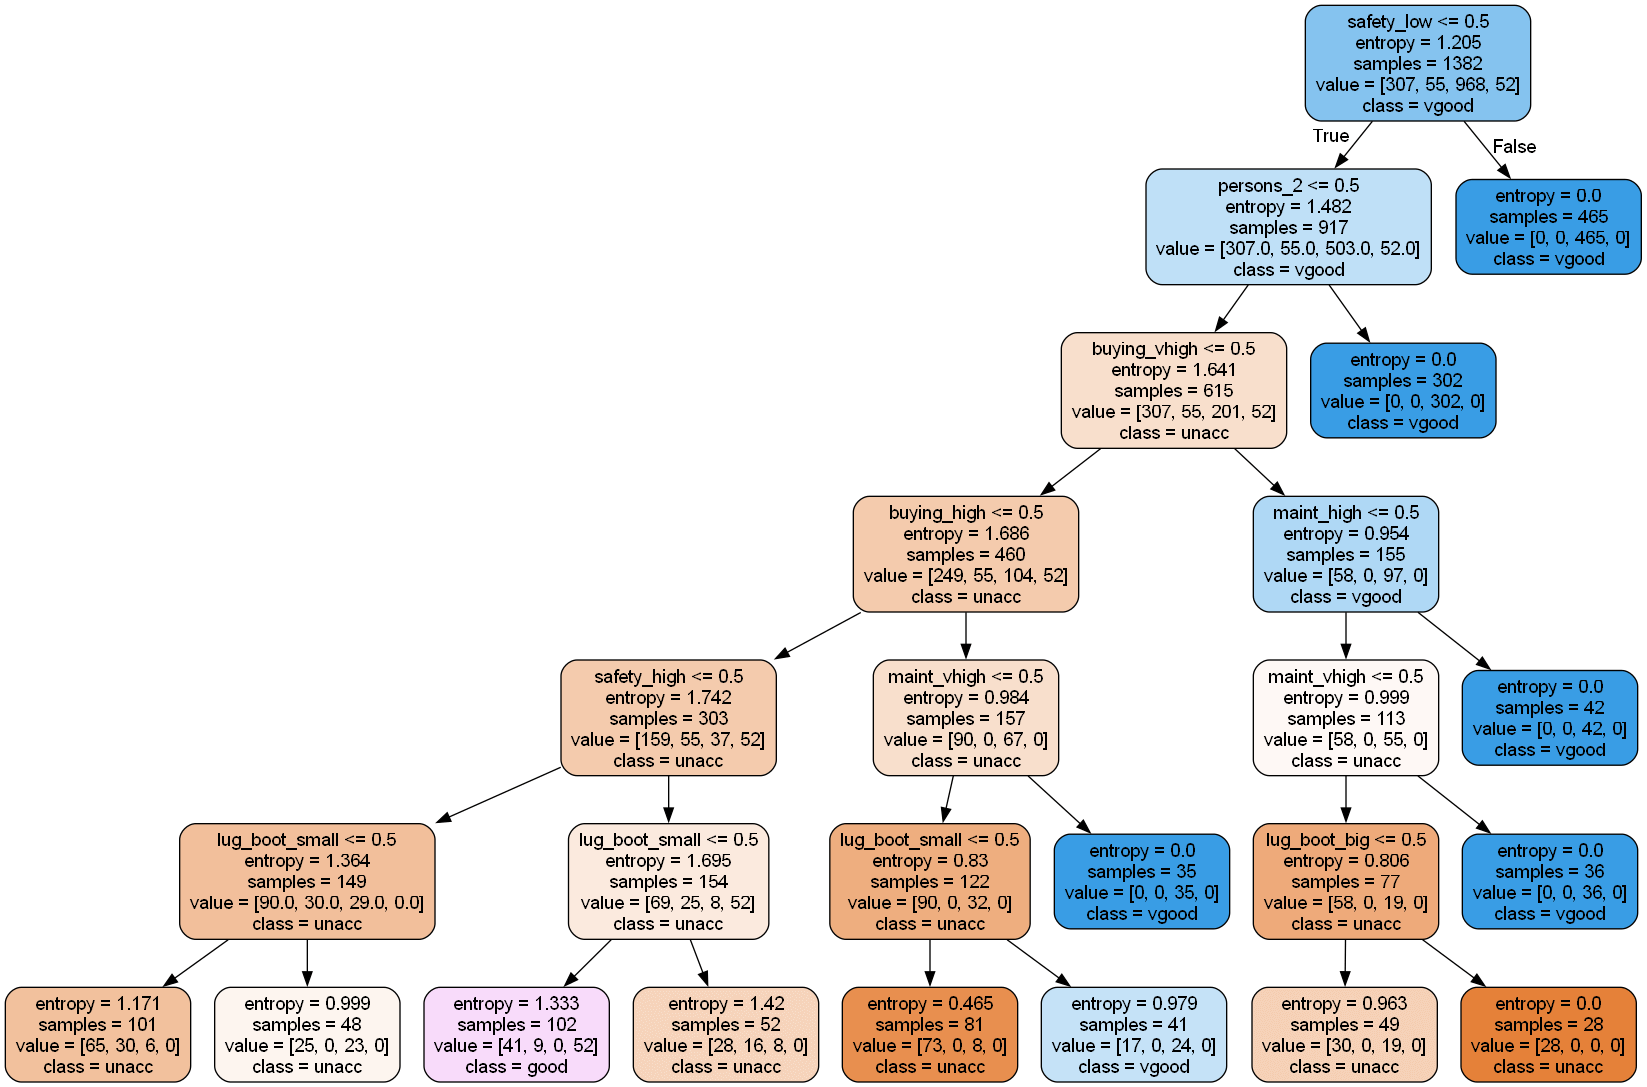
\includegraphics[width=0.8\textwidth]{imgs/dt-mini/dt__car_evaluation__80_vs_20__6.png}
	\caption{Car Evaluation: decision tree with \texttt{max\_depth}=6 (80/20 split).}\label{fig:ce-dt-depth-6}
\end{figure}

\begin{figure}[H]
	\centering
	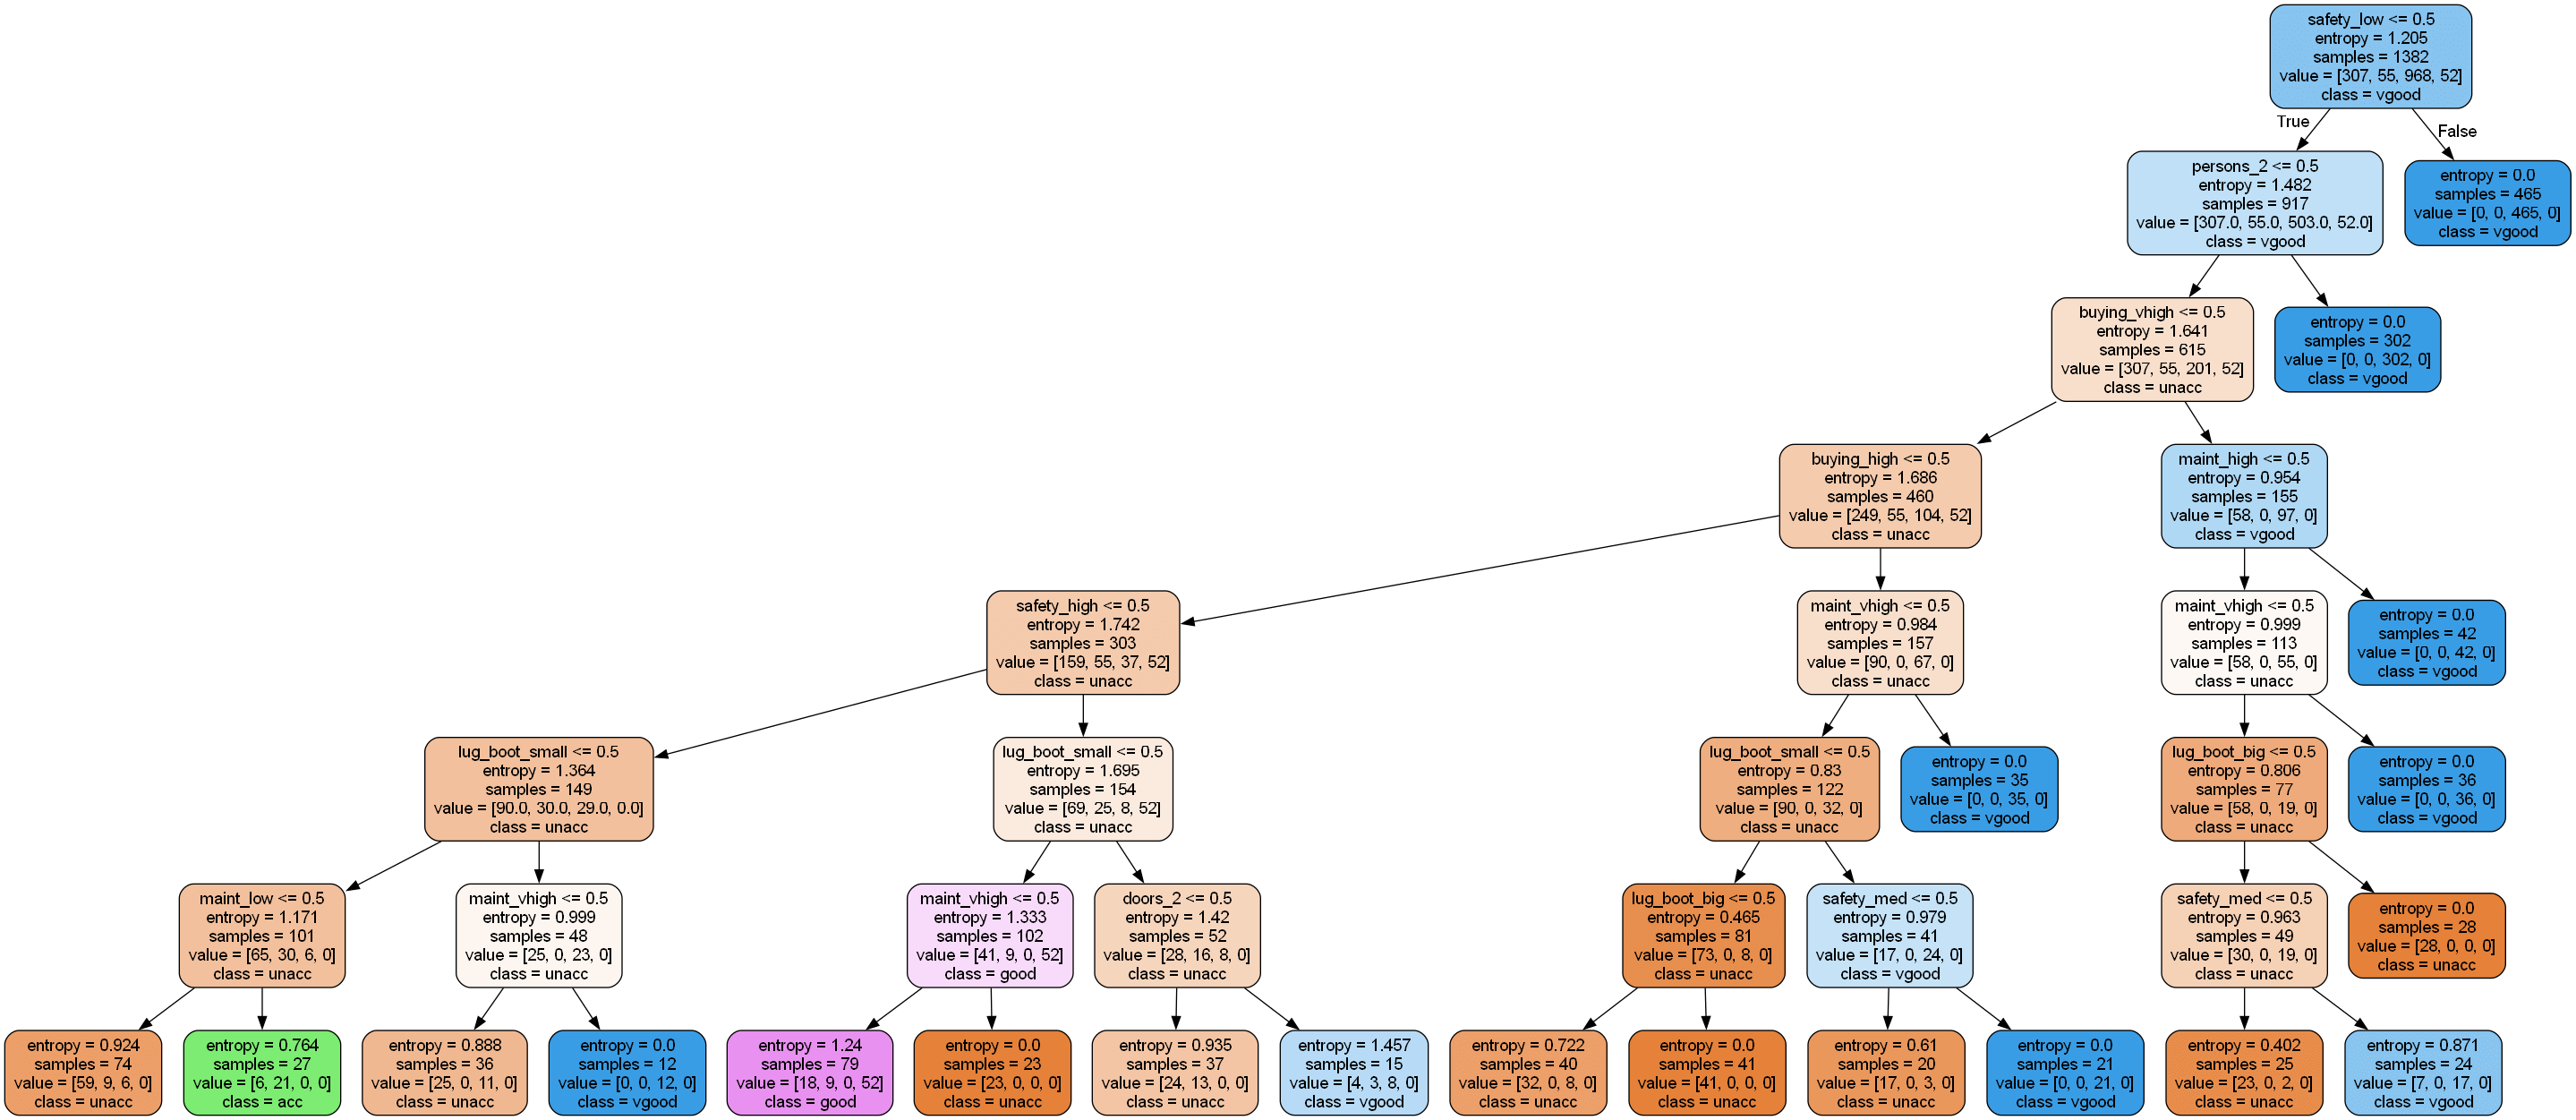
\includegraphics[width=0.8\textwidth]{imgs/dt-mini/dt__car_evaluation__80_vs_20__7.png}
	\caption{Car Evaluation: decision tree with \texttt{max\_depth}=7 (80/20 split).}\label{fig:ce-dt-depth-7}
\end{figure}

\begin{figure}[H]
	\centering
	\includegraphics[width=0.8\textwidth]{imgs/dt-mini/dt__car_evaluation__80_vs_20__None.png}
	\caption{Car Evaluation: decision tree with \texttt{max\_depth}=None (80/20 split).}\label{fig:ce-dt-depth-none}
\end{figure}

\section{Comparative Analysis}

\begin{itemize}
	\item \textbf{Objective:} Compare Decision Tree performance across:
	      \begin{enumerate}
		      \item Breast Cancer (binary classification, continuous features)
		      \item Wine Quality (multi-class, numerical features)
		      \item Car Evaluation (multi-class, categorical features)
	      \end{enumerate}

	\item \textbf{Comparison Criteria:}
	      \begin{itemize}
		      \item Accuracy, Precision, Recall, F1-Score
		      \item Effect of feature type and count
		      \item Class distribution and balance
		      \item Impact of \texttt{max\_depth} on overfitting
	      \end{itemize}

	\item \textbf{Observations:}
	      \begin{itemize}
		      \item \textbf{Breast Cancer:} Highest accuracy; binary labels and well-separated numeric features helped model performance.
		      \item \textbf{Wine Quality:} Lower precision for middle-quality wines; overlapping features across quality groups reduced clarity.
		      \item \textbf{Car Evaluation:} Performed well despite 4 classes; decision tree easily handled categorical data. Slight overfitting observed at deep trees.
	      \end{itemize}

	\item \textbf{Conclusion:}
	      \begin{itemize}
		      \item Decision Trees adapt well to both categorical and numerical data, but class imbalance and feature overlap affect performance.
		      \item Simpler datasets with clear boundaries (like Breast Cancer or Car Evaluation) yield higher accuracy.
		      \item Proper depth tuning is essential to maintain generalization.
	      \end{itemize}
\end{itemize}


% References
\pagebreak
\section{References}
\begin{enumerate}
  \item \href{https://scikit-learn.org/stable/modules/generated/sklearn.tree.DecisionTreeClassifier.html}{DecisionTreeClassifier Documentation}
  \item \href{https://scikit-learn.org/stable/modules/generated/sklearn.datasets.load_breast_cancer.html}{Breast Cancer Dataset}
  \item \href{https://scikit-learn.org/stable/modules/generated/sklearn.datasets.load_wine.html}{Wine Quality Dataset}
\end{enumerate}
\end{document}
